\appendix
\setcounter{section}{0}
\setcounter{subsection}{0}
\setcounter{subsubsection}{0}
\setcounter{table}{0}
\setcounter{figure}{0}
\renewcommand{\thesection}{S\arabic{section}}
\renewcommand{\thesubsection}{\thesection.\arabic{subsection}}
\renewcommand{\thesubsubsection}{\thesubsection.\arabic{subsubsection}}
\renewcommand{\thetable}{S\arabic{table}}
\renewcommand{\thefigure}{S\arabic{figure}}

\section{Supplementary Material}
\label{sec:supp}

This supplement documents GaitEval's single evaluation protocol: task-eligible participant partitions, label-redacted pose-derived evidence, declared model and evidence conditions, training-only fitting of supervised transformations, and fixed-task-label scoring with participant-aware interpretation. All six datasets---ASD-Kinect, ATAXIA, CARE-PD, GMFCS, PARKINSONISM, and PATHOGAIT---have equal benchmark membership. Model comparison, representation, adaptation, and transfer are experiment configurations within this protocol. Each result specifies its actual evaluation records and settings. The corrected GMFCS 866-clip participant maps are independently verified; complete training manifests for the seven-condition evaluation remain unavailable. The benchmark does not evaluate diagnosis from complete clinical records.

\subsection{Evaluation Scope, Resources, and Splits}
\label{sec:supp_scope}

\subsubsection{Evaluation records for model, view, and adaptation experiments}

Table~\ref{tab:core_resources} lists the larger-test records used for model, input-view, and adaptation experiments. Table~\ref{tab:standardized_contract} lists the seven-condition Qwen-7B records. Within each experiment, methods are compared on matching test IDs, labels, and feature columns. Tests with different eligible records are identified by their counts, not pooled as paired results. ATAXIA and PATHOGAIT concern performed patterns rather than patient-level diagnosis.

\begin{table}[H]
\centering
\caption{\textbf{Records for model, view, and adaptation experiments.} Walking clips in training/validation/test partitions. Dataset-specific tasks and participant counts determine interpretation. ``--'' means that this record configuration is not used for that dataset. Corrected GMFCS has 866 test clips for the verified five-model, SFT, and reference results; matching 7B view results remain unverified. The inconsistent historical 885-clip description is not an evaluation count.}
\label{tab:core_resources}
\small
\setlength{\tabcolsep}{3.5pt}
\begin{adjustbox}{max width=\textwidth}
\begin{tabular}{llllrrrl}
\toprule
Resource & Population/source & Task & Classes & Train & Val. & Test & Test subjects \\
\midrule
GMFCS & cerebral-palsy cohort; corrected split & ordinal severity & I--IV & 1,602 & 478 & 866 & 166 \\
ATAXIA & healthy volunteers performing ataxic gait & binary & normal / mimicked ataxia & 7,004 & 1,627 & 1,647 & 3 \\
PARKINSONISM & patient cohort & binary severity & mild / severe & 420 & 58 & 120 & 5 \\
PATHOGAIT & healthy volunteers performing six patterns & six-way pattern & normal + five abnormal patterns & 7,361 & 1,327 & 2,181 & 2 \\
ASD-Kinect & see next table & binary & ASD / typical & -- & -- & -- & -- \\
CARE-PD & see next table & UPDRS gait & 0--3 & -- & -- & -- & -- \\
\bottomrule
\end{tabular}
\end{adjustbox}
\end{table}

Subject identity is the uncertainty-resampling unit. ATAXIA's three model-comparison test participants contribute both normal and imitated-ataxia clips and are clustered across classes. PATHOGAIT has only two test participants, so no population-level superiority claim is made. The original GMFCS partition shared three patients between training and test (14 clips); checking validation identifies additional overlap. The repaired partition has 866 test clips from 166 participants and no participant intersections. The seven-condition GMFCS test has 255 clips from 149 participants. Original-to-corrected index maps preserve the provenance of the split-repair experiment.

\subsubsection{Evaluation records for the seven shared conditions}

The seven-condition evaluation uses one Qwen2.5-7B runner, prompt template, parser, and capture-quality-free feature policy across all six datasets (Table~\ref{tab:standardized_contract}). CARE-PD uses only the four-level UPDRS gait item: its full corpus has 362 patients and 8,476 clips, while this test subset has 665 clips from 24 patients. ASD-Kinect has a 70/10/20 participant split; the source reports some movements simulated by other people without identifying the affected sequences, so patient-only provenance is not independently established.

\begin{table}[H]
\centering
\caption{\textbf{Records and features for the seven shared conditions.} Feature counts reflect supported columns after skeleton-role mapping and removal of capture-quality variables. Test counts are the evaluable records in the released prediction files.}
\label{tab:standardized_contract}
\small
\setlength{\tabcolsep}{4pt}
\begin{tabular}{lrrrrl}
\toprule
Resource & Train clips & Test clips & Test subjects & Features & Label space \\
\midrule
ASD-Kinect & 70 & 20 & 20 & 23 & ASD / typical \\
ATAXIA & 28 & 8 & 4 & 14 & normal / mimicked ataxia \\
CARE-PD (UPDRS gait) & 1,901 & 665 & 24 & 24 & scores 0--3 \\
GMFCS & 914 & 255 & 149 & 16 & levels 1--4 \\
PARKINSONISM & 83 & 29 & 5 & 16 & mild / severe \\
PATHOGAIT & 5,040 & 1,440 & 2 & 24 & six gait patterns \\
\bottomrule
\end{tabular}
\end{table}

The shared-condition ATAXIA test has eight clips from four participants and supports descriptive conclusions only; the 1,647-clip model/adaptation test is a different recorded population. PARKINSONISM has 29 clips from five participants in the shared conditions and 120 clips from five participants in the model/adaptation experiments. Scores are compared only within their matching test records. CARE-PD score 3 has only 18 test clips, limiting class-specific interpretation.

\subsection{Pose Preprocessing and Model-Visible Input Views}
\label{sec:supp_inputs}

Each walking clip is converted into one model-visible view at a time. Views are never concatenated unless explicitly stated. Answer-revealing labels, sample identifiers, subject identifiers, and split metadata are removed from test-query evidence. Candidate classes define the task; few-shot references deliberately include their training labels.

\begin{table}[H]
\centering
\caption{\textbf{Controlled input representations.}
GaitEval uses four input-view families. The z-scored named-feature
representation is a derived scaling control within the named-feature
family. Motion summaries and feature
views are deterministic functions of the pose sequence.}
\label{tab:input_views}
\small
\begin{adjustbox}{max width=\textwidth}
\begin{tabular}{llll}
\toprule
View & Shape/format & Construction & Evaluation role \\
\midrule
Raw coordinates & $124\times J_d\times3$ & valid pose frames, zero-padded to fixed length & numeric-sequence stress test \\
Normalized coordinates & $32\times12\times3$ & common joints, body-centered, scale/direction normalized & cross-layout coordinate view \\
Motion summary & fixed-section English text & deterministic verbalization of measured features & primary readable evidence view \\
Raw feature vector & named values & supported biomechanical measurements & exact-feature evidence test \\
Z-scored named feature vector & named standardized values & training-mean/SD normalization & scale-controlled evidence test \\
\bottomrule
\end{tabular}
\end{adjustbox}
\end{table}

\subsubsection{Raw and normalized coordinate views}

Raw-coordinate experiment clips use a fixed tensor of $124$ frames by the dataset-specific joint count $J_d$ and three channels. Shorter clips are zero-padded; feature and summary computation uses only valid frames. At the nominal 30 frames/s, 124 frames correspond to approximately 4.1 seconds. Temporal measurements are expressed per frame or as dimensionless ratios so that no label-dependent temporal normalization is introduced.

The normalized coordinate view maps each skeleton to 12 common joints in the fixed order shoulders, elbows, wrists, hips, knees, and ankles. For every frame, the midpoint of the hips is subtracted from all joints. Coordinates are divided by the mean shoulder-center--to--hip-center distance computed over valid frames. The principal direction of the hip-center trajectory is aligned with the positive $x$ axis, and the remaining axes are defined by an orthogonal body-centered basis. Thirty-two frames are then selected at uniform temporal indices. The prompt contains a $32\times12\times3$ table rounded to two decimals. This view preserves relative motion while reducing differences in global location, scale, orientation, joint count, and clip duration.

\subsubsection{Deterministic biomechanical features}

For joint $j$, spatial channel $c$, and valid frame set $T$, range of motion is
\begin{equation}
R_{j,c}=\max_{t\in T}p_{t,j,c}-\min_{t\in T}p_{t,j,c}.
\end{equation}
Confidence channels are never used as spatial coordinates. For paired nonnegative measurements $v_L$ and $v_R$, unsigned asymmetry is
\begin{equation}
A(v_L,v_R)=\frac{|v_L-v_R|}{0.5(|v_L|+|v_R|)+10^{-8}}.
\end{equation}
The ratio lies in $[0,2]$ but discards the direction of asymmetry; this is a known limitation for unilateral presentations. The jerk proxy is the mean absolute third finite difference of the relevant trajectory. Trajectory variability is the temporal variance of the specified joint path. The standardized value is
\begin{equation}
z_{i,f}=\frac{x_{i,f}-\mu_f^{\mathrm{train}}}{\sigma_f^{\mathrm{train}}+10^{-8}},
\end{equation}
using training-split statistics only.

\begin{table}[H]
\centering
\caption{\textbf{Complete deterministic feature inventory.} Braces denote separate left and right features. Skeleton layouts that do not support a semantic role leave the corresponding feature undefined.}
\label{tab:feature_inventory}
\small
\begin{adjustbox}{max width=\textwidth}
\begin{tabular}{lll}
\toprule
Group & Released feature name & Definition \\
\midrule
Amplitude & \texttt{ankle\_\{L,R\}\_vert\_range} & vertical ankle range \\
Amplitude & \texttt{ankle\_\{L,R\}\_horiz\_range} & horizontal ankle range \\
Amplitude & \texttt{knee\_\{L,R\}\_vert\_range} & vertical knee range \\
Amplitude & \texttt{hip\_\{L,R\}\_vert\_range} & vertical hip range \\
Asymmetry & \texttt{ankle\_vert\_asymmetry} & paired ankle vertical-range asymmetry \\
Asymmetry & \texttt{ankle\_horiz\_asymmetry} & paired ankle horizontal-range asymmetry \\
Asymmetry & \texttt{knee\_vert\_asymmetry} & paired knee vertical-range asymmetry \\
Asymmetry & \texttt{hip\_vert\_asymmetry} & paired hip vertical-range asymmetry \\
Stability & \texttt{trunk\_lateral\_sway} & lateral trunk range \\
Stability & \texttt{trunk\_vert\_range} & vertical trunk range \\
Stability & \texttt{hip\_centre\_lateral\_std} & lateral hip-center standard deviation \\
Stability & \texttt{hip\_centre\_vert\_std} & vertical hip-center standard deviation \\
Variability & \texttt{mean\_joint\_trajectory\_var} & mean joint-path variance \\
Variability & \texttt{ankle\_\{L,R\}\_traj\_var} & left/right ankle-path variance \\
Smoothness & \texttt{ankle\_\{L,R\}\_jerk} & left/right ankle jerk proxy \\
Smoothness & \texttt{ankle\_mean\_jerk} & mean of the ankle jerk proxies \\
Smoothness & \texttt{trunk\_jerk} & trunk jerk proxy \\
Capture audit & \texttt{valid\_frame\_fraction} & fraction of valid frames in the fixed tensor \\
\bottomrule
\end{tabular}
\end{adjustbox}
\end{table}

The inventory above describes the coordinate-derived extractor, with 23 motion measurements and the capture-quality field \texttt{valid\_frame\_fraction}. Supported feature columns depend on skeleton layout. The seven shared conditions use 14/16/16/24/23/24 features for ATAXIA/GMFCS/PARKINSONISM/PATHOGAIT/ASD-Kinect/CARE-PD and exclude capture-quality variables, including clip length and valid-frame fraction. The larger-test model/view/adaptation inputs retain their recorded supported columns; the explicit PATHOGAIT field-removal experiment quantifies its effect on matching IDs. Missing joints are omitted from both LLM and reference inputs. Reference models impute supported missing values with training medians; text prompts omit undefined values. Complete feature CSVs remain external, so identical columns across different experiments are not assumed.

\subsubsection{Motion-summary provenance and template}
\label{sec:supp_summary_provenance}

Motion summaries are deterministic, label-independent renderings of the selected feature vector, not annotations or outputs of another language model. Sections follow \textsc{Motion amplitude}, \textsc{Symmetry/asymmetry}, \textsc{Stability}, \textsc{Trajectory variability}, and \textsc{Smoothness}. The larger-test summary generator additionally emits a \textsc{Clip quality} line. This line and its underlying feature are excluded from all seven shared conditions; the feature-removal experiment separately evaluates the 2,181-clip PATHOGAIT record set.

Raw amplitudes and ranges are printed to four decimals; variances and jerk proxies are printed to six decimals. A small set of fixed thresholds adds qualitative wording without using a label:
\begin{itemize}
\item asymmetry $<0.05$: symmetric; $[0.05,0.15)$: mild; $[0.15,0.30)$: notable; $\geq0.30$: strong;
\item trunk lateral sway $<0.04$: mild; $[0.04,0.09)$: moderate; $\geq0.09$: marked;
\item ankle mean jerk $<2\times10^{-4}$: smooth; $[2\times10^{-4},8\times10^{-4})$: moderately smooth; $\geq8\times10^{-4}$: jerky.
\end{itemize}
The thresholds only select descriptive phrases; the underlying numerical values are retained. A typical summary is 150--300 words (approximately 320 tokens). The following schematic preserves the exact structure while using illustrative values:

\begin{quote}\small\ttfamily
MOTION AMPLITUDE\par
Left/right ankle vertical range: 0.0900 / 0.1400.\par
Left/right knee vertical range: 0.0710 / 0.0840.\par
\medskip
SYMMETRY/ASYMMETRY\par
Ankle vertical asymmetry: 0.4350 (strong asymmetry).\par
\medskip
STABILITY\par
Trunk lateral sway: 0.0400 (moderate sway).\par
\medskip
TRAJECTORY VARIABILITY\par
Mean joint trajectory variance: 0.008000.\par
\medskip
SMOOTHNESS\par
Mean ankle jerk: 0.000700 (moderately smooth).\par
\end{quote}

The candidate label set is inserted only by the downstream classification prompt. It is never available to the summary generator, so the motion evidence and task instruction remain separate objects.

\subsection{Exact Prompt Formats and Output Parsing}
\label{sec:supp_prompts}

\subsubsection{Flat zero-shot prompt}

The shared-condition flat-prompt template is instantiated as follows (line wrapping is for display), where bracketed fields are filled with the selected evidence view and the dataset's complete candidate list:

\begin{Verbatim}[fontsize=\small,frame=single]
You are classifying a gait clip from a compact biomechanical
[EVIDENCE_KIND] derived from a skeleton sequence.

[EVIDENCE]

Task: based ONLY on the [EVIDENCE_KIND] above, classify the gait
into exactly one of the following classes:
- [CLASS 1]
- [CLASS 2]
...

Return only one label, written exactly as listed above.
\end{Verbatim}

For motion summaries, \texttt{EVIDENCE\_KIND} is ``motion summary''; for raw or z-scored features it is ``feature description.'' The larger-test view experiments use the recorded 3D-skeleton/biomechanical-dimension preamble. These template settings are documented with the experiment, and do not supply clinical definitions, prevalence, demonstrations, or answer labels in zero-shot queries.


\subsubsection{Reasoning-anchored prompt}

The reasoning-anchored condition used the same label-redacted motion
summary as the flat condition, but replaced the direct-answer
instruction with the following structured prompt. No separate system
message was used; the complete prompt was sent as a single user
message. Bracketed fields below denote deterministic run-time
substitutions.

\begin{Verbatim}[fontsize=\scriptsize,frame=single,breaklines=true,breakanywhere=true]
You are a gait-analysis expert classifying a walking clip from a compact biomechanical motion summary derived from a 3D skeleton sequence. The summary reports motion amplitudes, left/right asymmetry, trunk/pelvis stability, trajectory variability, and movement smoothness (jerk).

[MOTION_SUMMARY]

Candidate classes:
[CANDIDATE_CLASS_LINES]

Reason step by step:
1. List the 2-3 most abnormal biomechanical signals in this summary (e.g. high asymmetry, high jerk, large trunk sway, reduced amplitude).
2. For EACH candidate class, briefly state whether those signals are consistent or inconsistent with it.
3. Do NOT default to the most common class; pick the class best supported by the specific signals.
Finally, on a new line, output exactly: FINAL: <one class name>
\end{Verbatim}

The candidate lines were inserted in ascending numeric-label order
using the exact dataset label strings. This condition used
Qwen2.5-72B-Instruct with temperature~0 and a maximum of 512 output
tokens. For ATAXIA and PATHOGAIT, the test records were shuffled with
seed~0 before selecting 150 clips. PARKINSONISM contains only 120 test
clips, so all of its test clips were evaluated after the same seeded
shuffle. The generated reasoning text was not treated as explanation
supervision or scored for clinical correctness; only the parsed final
class was evaluated.

For the three evaluated resources, the exact candidate strings were:
\begin{itemize}
    \item ATAXIA: \texttt{normal gait};
    \texttt{cerebellar ataxic gait}.
    \item PARKINSONISM: \texttt{low motor severity};
    \texttt{high motor severity}.
    \item PATHOGAIT: \texttt{normal gait};
    \texttt{antalgic gait}; \texttt{lurching gait};
    \texttt{steppage gait}; \texttt{stiff-legged gait};
    and \texttt{Trendelenburg gait}.
\end{itemize}




\subsubsection{Few-shot prompt}

Few-shot prompting was implemented as one user message containing a
sequence of labeled textual reference blocks, followed by the
unlabeled test query. It was not implemented as a multi-turn sequence
of separate user and assistant messages. No separate system message
was used. The literal template was:

\begin{Verbatim}[fontsize=\scriptsize,frame=single,breaklines=true]
You are classifying a gait clip from a compact biomechanical motion summary derived from a 3D skeleton sequence. Feature values (amplitudes, left/right asymmetry, stability, trajectory variability, smoothness) must be judged RELATIVE TO THIS DATASET, not by generic clinical intuition. Below are [N_SHOTS] labeled reference clips from the same dataset and feature pipeline; use them to calibrate what each class looks like here.

=== Reference example 1 ===
[REFERENCE_MOTION_SUMMARY_1]
Ground-truth class: [REFERENCE_CLASS_1]

=== Reference example 2 ===
[REFERENCE_MOTION_SUMMARY_2]
Ground-truth class: [REFERENCE_CLASS_2]

[ADDITIONAL_REFERENCE_BLOCKS]

=== Now classify this new clip ===
[QUERY_MOTION_SUMMARY]

Candidate classes:
[CANDIDATE_CLASS_LINES]

Return only one label, written exactly as listed above.
\end{Verbatim}

Reference examples were drawn only from the dataset's training split.
For a requested context size $k$ and $C$ classes, the implementation
grouped training examples by numeric class, shuffled each class pool
with seed~0, selected
$\max(1,\lfloor k/C\rfloor)$ examples from each class, and then
shuffled the combined reference set using the same random-number
generator. All reported context sizes were divisible by the
corresponding number of classes, so the realized reference set
contained exactly $k$ examples and was class-balanced. One fixed
reference set was reused for every test clip within a run.

Inference used Qwen2.5-72B-Instruct, temperature~0, a maximum of
64 output tokens, and the same exact-label parser used for the corresponding
flat-prompt experiments.

The reported settings were:
\begin{itemize}
    \item ATAXIA: $k\in\{8,16,32\}$, corresponding to
    4, 8, and 16 references per class, evaluated on the full test
    split.
    \item PARKINSONISM: $k=16$, corresponding to 8 references per
    class, evaluated on the full test split.
    \item PATHOGAIT: $k=12$, corresponding to 2 references per class.
    This run evaluated the first 600 records in the stored test-file
    order rather than the complete 2,181-clip test split.
\end{itemize}

\subsubsection{Parser and invalid outputs}

The reasoning condition did not use a dedicated parser for the
\texttt{FINAL:} field. The reasoning and few-shot outputs were parsed
with the same exact-label parser as the corresponding flat-prompt
runs. Outputs were whitespace-normalized and lowercased, and candidate
strings were matched with leading and trailing alphanumeric
boundaries. When several complete candidate strings occurred, the
latest occurrence was selected; positional ties favored the longer
candidate string. Consequently, a compliant final
\texttt{FINAL: <class>} line was normally selected because it was the
last candidate mention, rather than because the parser explicitly
recognized the \texttt{FINAL:} prefix.

If no complete candidate occurred, the larger-test view/few-shot implementation additionally
accepted an output-ending substring only when it was a unique prefix
of exactly one candidate label, providing a limited fallback for
truncated generations. All other outputs were marked
\texttt{UNPARSED}. Unparsed outputs were never discarded: they were
counted as errors and contributed a false negative to the true class.

\subsection{Models, Inference, and Adaptation}
\label{sec:supp_models}

\subsubsection{Zero-shot model roster}

The five-model motion-summary experiment uses Llama-3.3-70B-Instruct, Qwen2.5-72B-Instruct, Gemma-3-27B-IT, GLM-4-32B-0414, and DeepSeek-R1-Distill-Qwen-32B. All use deterministic decoding through vLLM. Test clips are 20, 1,647, 665, 866, 120, and 2,181 for ASD-Kinect, ATAXIA, CARE-PD, GMFCS, PARKINSONISM, and PATHOGAIT. The shared-condition evaluation instead uses Qwen2.5-7B on 20/8/665/255/29/1,440 clips, as listed in the evaluation-record tables.

Generation limits are recorded per experiment: the shared-condition Qwen-7B runs and ASD-Kinect/CARE-PD non-reasoning model runs use 48 tokens; the larger-test view launcher uses 16; the other direct-answer model and few-shot runs use 64. Reasoning-distilled runs use 2,048 tokens. All use temperature 0. Few-shot and reasoning-anchored probes use Qwen2.5-72B. The larger-test parser has a unique truncated-prefix fallback, while the seven-condition parser requires complete candidate mentions. These settings preclude matched-budget or identical-parser claims across different experiments. Within each summary-SFT comparison, its zero-shot and SFT prompts are byte-identical.

\subsubsection{LoRA supervised fine-tuning}

For the seven shared conditions, LoRA-SFT is trained separately for each dataset on training-split motion summaries and their candidate labels. The configuration is rank $r=16$, scaling $\alpha=32$, dropout 0.05, and adapters on all linear projections. Training uses completion-only cross-entropy, three epochs, learning rate $10^{-4}$ with cosine decay, maximum sequence length 1,024, per-device batch size 8, and gradient accumulation 2 (effective batch size 16). The committed trainer reads only training examples, uses no evaluation dataset and no intermediate checkpoint selection (\texttt{save\_strategy="no"}), and saves the final three-epoch adapter. A validation-selected checkpoint is not supported by this implementation. The configured test split is not used for training or normalization.

The shared-condition training-set sizes are 28 for ATAXIA, 914 for GMFCS, 83 for PARKINSONISM, 5,040 for PATHOGAIT, 70 for ASD-Kinect, and 1,901 for CARE-PD. CARE-PD training examples are restricted to the UPDRS gait task. SFT therefore measures recovery of an in-distribution, dataset-specific mapping from supplied evidence to the dataset label space; it is not interpreted as acquisition of a general diagnostic rule.

\subsubsection{Few-shot sweep}

\begin{table}[H]
\centering
\caption{\textbf{Few-shot motion-summary prompting.} Qwen2.5-72B receives balanced labeled training examples. Cells report accuracy / macro-F1 / Cohen's $\kappa$. Bold marks the best tested context size within a dataset.}
\label{tab:fewshot_sweep}
\small
\begin{tabular}{lll}
\toprule
Dataset & Setting & Accuracy / macro-F1 / $\kappa$ \\
\midrule
ATAXIA & zero-shot & 0.685 / 0.406 / $-0.002$ \\
ATAXIA & $k=8$ & 0.682 / 0.644 / 0.289 \\
ATAXIA & $k=16$ & \textbf{0.740 / 0.697 / 0.395} \\
ATAXIA & $k=32$ & 0.642 / 0.633 / 0.299 \\
\addlinespace
PARKINSONISM & zero-shot & 0.575 / 0.472 / 0.035 \\
PARKINSONISM & $k=16$ & \textbf{0.567 / 0.561 / 0.188} \\
\addlinespace
PATHOGAIT & zero-shot & 0.155 / 0.055 / $-0.009$ \\
PATHOGAIT & $k=12$ & \textbf{0.268 / 0.185 / 0.081} \\
\bottomrule
\end{tabular}
\end{table}

The ATAXIA curve is non-monotonic, so few-shot prompting is treated as an adaptation probe rather than a tuned final model. PATHOGAIT uses two references per class at $k=12$, but its 600-clip few-shot subset differs from the 2,181-clip zero-shot row; their difference is not a paired full-test gain.

\subsection{Matched Linear References}
\label{sec:supp_references}

The supervised references are multinomial or binary logistic regression and a linear support-vector machine. Both receive exactly the supported deterministic feature columns available to the feature-view LLM condition. The supervised references use prespecified estimator settings:
logistic regression is fitted with \texttt{max\_iter=2000}, and the
linear SVM with \texttt{max\_iter=5000}. The class-balanced
configuration is the primary reference, while the unweighted
configuration is reported as a parallel sensitivity analysis rather
than selected on validation performance. Missing values are imputed
using training-set medians, and the imputer and standard scaler are
fitted on the training split only before being applied to the held-out
test split. No validation-based hyperparameter search is performed. Columns missing for an entire dataset are dropped, and residual missing values are imputed with the training median. These models are signal probes: they establish whether the deterministic pose representation contains label-relevant information under supervised learning, rather than representing the state of the art in clinical gait analysis.

\begin{table}[H]
\centering
\caption{\textbf{Feature-reference weighting check on the larger-test records.} ``--'' denotes no result. Macro-F1 on the specified model/adaptation test sets. ``Balanced'' uses inverse-frequency class weights; ``none'' uses the empirical training distribution.}
\label{tab:core_linear_refs}
\small
\begin{tabular}{lrrrr}
\toprule
Reference & ATAXIA & GMFCS & PARKINSONISM & PATHOGAIT \\
\midrule
Logistic regression (balanced) & 0.763 & 0.395 & 0.613 & 0.662 \\
Logistic regression (none) & 0.773 & 0.418 & 0.627 & 0.663 \\
Linear SVM (balanced) & 0.759 & 0.412 & 0.583 & 0.644 \\
Linear SVM (none) & 0.768 & 0.400 & 0.579 & 0.646 \\
ASD-Kinect & -- & -- & -- & -- \\
CARE-PD & -- & -- & -- & -- \\
\bottomrule
\end{tabular}
\end{table}

On the 2,181-clip PATHOGAIT test, removing \texttt{valid\_frame\_fraction} reduces balanced LR macro-F1 from 0.662 to 0.564 and linear-SVM macro-F1 from 0.644 to 0.560. A pre-repair sensitivity check recorded changes below 0.001 for the other tested resources, but does not establish that bound for corrected GMFCS. The feature-SFT results are therefore interpreted using their supplied measurements, without a kinematics-only claim. The seven shared conditions exclude capture-quality variables for all methods.

\subsection{Metrics and Statistical Analysis}
\label{sec:supp_metrics}

Let $C_{ab}$ denote the number of clips whose true class is $a$ and
predicted class is $b$, for a fixed candidate set of $K$ classes.
Let $u_a$ count invalid predictions for true class $a$, so $N=\sum_{a,b=1}^{K}C_{ab}+\sum_{a=1}^{K}u_a$. For class $k$, precision, recall, and F1 are
\begin{equation}
P_k=\frac{C_{kk}}{\sum_{a=1}^{K}C_{ak}},\qquad
R_k=\frac{C_{kk}}{\sum_{b=1}^{K}C_{kb}+u_k},
\end{equation}
and
\begin{equation}
F_{1,k}=\frac{2P_kR_k}{P_k+R_k}.
\end{equation}
A metric is set to zero when its denominator is zero. Macro-F1 is the
unweighted mean over the complete dataset-defined class set,
\begin{equation}
\operatorname{MacroF1}
    =\frac{1}{K}\sum_{k=1}^{K}F_{1,k},
\end{equation}
including classes that receive no predictions. Accuracy is
\begin{equation}
\operatorname{Accuracy}
    =\frac{1}{N}\sum_{k=1}^{K}C_{kk}.
\end{equation}
These metrics are reported together because accuracy alone can obscure
class-allocation failures on imbalanced tasks
\cite{opitz2019macro,sokolova2009performance}.

For binary tasks, sensitivity is recall for the dataset-specified
positive class, whereas specificity is recall for the complementary
negative class. Balanced accuracy is
\begin{equation}
\operatorname{BalancedAccuracy}
    =\frac{\operatorname{Sensitivity}
            +\operatorname{Specificity}}{2}.
\end{equation}

Cohen's agreement coefficient is
\begin{equation}
\kappa=\frac{p_o-p_e}{1-p_e},
\qquad
p_o=\frac{1}{N}\sum_{i=1}^{N}
        \mathbf{1}(y_i=\hat y_i),
\end{equation}
where $y_i$ and $\hat y_i$ are the true and parsed predicted labels for
clip $i$. Chance agreement is computed from the empirical target and
prediction marginals:
\begin{equation}
p_e=\sum_{k=1}^{K}
\left(\frac{n_k^{(y)}}{N}\right)
\left(\frac{n_k^{(\hat y)}}{N}\right),
\end{equation}
where $n_k^{(y)}$ and $n_k^{(\hat y)}$ are the numbers of true and
predicted instances of class $k$, respectively
\cite{cohen1968weighted}. An unparsed output is assigned a
prediction-only sentinel category outside the candidate set. It is
therefore always incorrect, contributes a false negative to its true
class, and cannot create a true positive for any candidate class.

For ordinal GMFCS and CARE-PD tasks, mean absolute error (MAE) is
computed over the ordered class indices:
\begin{equation}
\operatorname{MAE}
    =\frac{1}{N}\sum_{i=1}^{N}
       \left|r(y_i)-r(\hat y_i)\right|,
\end{equation}
where $r(\cdot)$ maps a class label to its ordinal level. We additionally
report quadratic-weighted Cohen's $\kappa$. Let
\begin{equation}
w_{ab}=\frac{(a-b)^2}{(K-1)^2}
\end{equation}
be the quadratic disagreement weight, $O_{ab}=C_{ab}$ the observed
confusion matrix, and
\begin{equation}
E_{ab}=\frac{n_a^{(y)}n_b^{(\hat y)}}{N}
\end{equation}
the expected count under independent target and prediction marginals.
Quadratic-weighted agreement is
\begin{equation}
\kappa_{\mathrm{q}}
    =1-\frac{\sum_{a=1}^{K}\sum_{b=1}^{K}w_{ab}O_{ab}}
             {\sum_{a=1}^{K}\sum_{b=1}^{K}w_{ab}E_{ab}}.
\end{equation}
This metric gives larger penalties to errors spanning more ordinal
levels. The three plotted ordinal conditions have no invalid outputs; MAE and weighted agreement are reported only for those valid ordered-label cells. Per-class metrics and confusion matrices cover the three plotted conditions, rather than every control condition.

Uncertainty is primarily quantified using a participant-cluster
bootstrap with $B=2{,}000$ draws. For each draw, the test participants
are sampled with replacement, and all clips from each sampled
participant are retained together. The metric is recomputed on every
valid draw (at least two distinct participants and two true classes), and the 2.5th and 97.5th percentiles form the 95\%
confidence interval \cite{efron1993bootstrap}. For a paired comparison,
the same sampled participants and matched clips are used for both
conditions. If
\begin{equation}
\Delta=T_A-T_B
\end{equation}
is the observed macro-F1 difference, the paired confidence interval is
obtained from the bootstrap distribution of $\Delta^{*}$. The reported
two-sided paired $p$ value is estimated from the proportions of
participant-bootstrap differences on the two sides of zero. These
paired tail areas summarize changes while preserving within-participant dependence. Point metrics here retain the fixed task label set. The archived bootstrap code instead uses the union of observed true/predicted labels, including an invalid-output sentinel and omitting absent classes. Thus, its intervals and tail areas are historical diagnostics, not independently regenerated fixed-label uncertainty estimates.

The per-cell permutation-against-chance values in the shared-condition grid
use a separate row-level label-permutation test. The true labels are
permuted relative to the fixed predictions while preserving their
empirical marginal counts. With observed statistic $T_{\mathrm{obs}}$
and permuted statistics $T^{(b)}$, the one-sided Monte Carlo value is
\begin{equation}
p_{\mathrm{perm}}
  =\frac{1+\sum_{b=1}^{B}
       \mathbf{1}\!\left(T^{(b)}\geq T_{\mathrm{obs}}\right)}
       {B+1}.
\end{equation}
With $B=2{,}000$, the minimum attainable value is approximately
$0.0005$. Because this permutation operates on individual records
rather than participant clusters, it is treated as a descriptive null
comparison and not as participant-level population inference. The archived cluster intervals and paired tail areas retain their stated historical metric convention. The shared-condition permutation calculations use 2,000 draws; reference-table values from the larger-test experiments are retained at their source precision rather than assigned the same Monte Carlo budget.

The limited numbers of independent participants constrain these
analyses. The larger-test ATAXIA and PARKINSONISM test sets contain three and
five participants, respectively. PATHOGAIT contains only two test
participants, for which participant-cluster resampling is degenerate;
its frozen-split results are therefore reported as descriptive point
estimates with participant-specific values and are not used to support
population-level superiority. ASD-Kinect contains one clip per
participant, so record-level and participant-level resampling coincide.
The highest GMFCS and CARE-PD ordinal levels also have small supports
and should be interpreted jointly with their per-class results and
confusion matrices.

\subsection{Five-Model Zero-Shot Results}
\label{sec:supp_primary_zero}

Table~\ref{tab:primary_five_family} gives the full five-model motion-summary results on the test sets listed in its caption. Across the 1,647/866/120/2,181-clip ATAXIA/GMFCS/PARKINSONISM/PATHOGAIT tests, $\kappa$ ranges from $-0.069$ to 0.043 after the GMFCS repair. CARE-PD and ASD-Kinect have their own reported ranges. Dominant-class shares show that high accuracy can coexist with concentrated outputs. PATHOGAIT Llama/GLM macro-F1 is .062/.069 over six task labels; earlier .053/.059 values averaged an extra invalid-output category. Invalid responses continue to count as errors.

\begin{table}[H]
\centering
\caption{\textbf{Five-model zero-shot motion-summary results.} Accuracy / macro-F1 / Cohen's $\kappa$; top share is the dominant predicted-class fraction. Test clips in dataset order ASD-Kinect, ATAXIA, CARE-PD, GMFCS, PARKINSONISM, and PATHOGAIT are 20/1,647/665/866/120/2,181. GMFCS uses the corrected test participants. These are model-comparison records; the seven-condition evaluation's counts are specified separately in the evaluation-record inventory.}
\label{tab:primary_five_family}
\scriptsize
\begin{adjustbox}{max width=\textwidth}
\begin{tabular}{llrrrr}
\toprule
Dataset & Model & Accuracy & Macro-F1 & $\kappa$ & Top share \\
\midrule
ATAXIA & Llama-3.3-70B & 0.686 & 0.407 & 0.000 & 1.00 \\
& Qwen2.5-72B & 0.685 & 0.406 & $-0.002$ & 1.00 \\
& Gemma-3-27B & 0.686 & 0.407 & 0.000 & 1.00 \\
& GLM-4-32B & 0.686 & 0.407 & 0.000 & 1.00 \\
& DeepSeek-R1-Distill-Qwen-32B & 0.684 & 0.408 & $-0.002$ & 1.00 \\
\addlinespace
GMFCS & Llama-3.3-70B & 0.353 & 0.212 & 0.025 & 0.72 \\
& Qwen2.5-72B & 0.372 & 0.222 & 0.043 & 0.78 \\
& Gemma-3-27B & 0.313 & 0.163 & 0.030 & 0.86 \\
& GLM-4-32B & 0.269 & 0.127 & $-0.000$ & 0.93 \\
& DeepSeek-R1-Distill-Qwen-32B & 0.311 & 0.191 & 0.014 & 0.64 \\
\addlinespace
PARKINSONISM & Llama-3.3-70B & 0.583 & 0.368 & 0.000 & 1.00 \\
& Qwen2.5-72B & 0.575 & 0.472 & 0.035 & 0.86 \\
& Gemma-3-27B & 0.583 & 0.368 & 0.000 & 1.00 \\
& GLM-4-32B & 0.583 & 0.368 & 0.000 & 1.00 \\
& DeepSeek-R1-Distill-Qwen-32B & 0.583 & 0.368 & 0.000 & 1.00 \\
\addlinespace
PATHOGAIT & Llama-3.3-70B & 0.159 & 0.062 & $-0.010$ & 0.94 \\
& Qwen2.5-72B & 0.155 & 0.055 & $-0.009$ & 0.94 \\
& Gemma-3-27B & 0.165 & 0.047 & $-0.001$ & 1.00 \\
& GLM-4-32B & 0.141 & 0.069 & $-0.069$ & 0.51 \\
& DeepSeek-R1-Distill-Qwen-32B & 0.166 & 0.094 & $-0.007$ & 0.48 \\
ASD-Kinect & Llama-3.3-70B & 0.500 & 0.451 & 0.000 & 0.80 \\
 & Qwen2.5-72B & 0.450 & 0.373 & -0.100 & 0.85 \\
 & Gemma-3-27B & 0.450 & 0.310 & -0.100 & 0.95 \\
 & GLM-4-32B & 0.450 & 0.373 & -0.100 & 0.85 \\
 & DeepSeek-R1-Distill-Qwen-32B & 0.600 & 0.583 & 0.200 & 0.70 \\
CARE-PD & Llama-3.3-70B & 0.441 & 0.262 & 0.119 & 0.71 \\
 & Qwen2.5-72B & 0.445 & 0.268 & 0.129 & 0.64 \\
 & Gemma-3-27B & 0.439 & 0.249 & 0.113 & 0.72 \\
 & GLM-4-32B & 0.441 & 0.350 & 0.124 & 0.56 \\
 & DeepSeek-R1-Distill-Qwen-32B & 0.398 & 0.295 & 0.099 & 0.45 \\
\bottomrule
\end{tabular}
\end{adjustbox}
\end{table}

These results bound the primary claim: the evaluated off-the-shelf models do not consistently ground dataset labels in the supplied motion summaries. They do not imply that pose contains no signal or that every possible language-model representation must fail.

\subsection{Representation and Prompt Controls}
\label{sec:supp_controls}

\subsubsection{Same-model view comparison}

Table~\ref{tab:core_views} reports the Qwen2.5-7B view experiment on 20/1,647/665/866/120/2,181 test clips in dataset order. Red GMFCS entries are displayed for author review only: the summary value comes from a logged 866-clip cross-stack run, normalized coordinates from an unverified source draft, and both feature values from 899-clip aggregates. They do not establish a matched-test comparison and are excluded from scientific comparisons. No view is consistently successful across the tested populations. In the seven-condition evaluation, PARKINSONISM
z-scored feature view reaches 0.757 macro-F1 on 29 clips from five
participants (Table~\ref{tab:standardized_full_grid}). This result
indicates that evidence use can depend on both the dataset and the input
representation, although the small test cohort precludes a broad
population-level conclusion.

\begin{table}[H]
\centering
\caption{\textbf{Qwen2.5-7B zero-shot input-view experiment.} Accuracy / macro-F1 / $\kappa$ on 20/1,647/665/866/120/2,181 clips in dataset order ASD-Kinect, ATAXIA, CARE-PD, GMFCS, PARKINSONISM, and PATHOGAIT. ``--'' denotes no recoverable numeric result. \textcolor{red}{Red denotes additions for author review. GMFCS summary is log-only (866 clips); normalized coordinates are draft-only/unverified; raw/z-scored features use 899 clips. These are not verified matched-test results. PATHOGAIT raw features use a recovered 2,181-clip recompute aggregate.} The record audit is below. The seven-condition test sets have their own input-view table.}
\label{tab:core_views}
\scriptsize
\begin{adjustbox}{max width=\textwidth}
\begin{tabular}{lrrrr}
\toprule
Dataset & Motion summary & Normalized coordinates &
Raw feature view & Z-scored feature view \\
\midrule
ATAXIA & 0.692 / 0.452 / 0.046 & 0.316 / 0.244 / 0.002 & 0.382 / 0.347 / 0.057 & 0.583 / 0.495 / $-0.008$ \\
GMFCS & \textcolor{red}{0.259 / 0.113 / $-0.009$} & \textcolor{red}{0.282 / 0.110 / 0.000} & \textcolor{red}{0.343 / 0.245 / 0.007} & \textcolor{red}{0.185 / 0.100 / $-0.049$} \\
PARKINSONISM & 0.550 / 0.400 / $-0.045$ & 0.442 / 0.441 / $-0.095$ & 0.417 / 0.294 / 0.000 & 0.508 / 0.493 / $-0.014$ \\
PATHOGAIT & 0.142 / 0.087 / $-0.024$ & 0.110 / 0.034 / 0.000 & \textcolor{red}{0.110 / 0.033 / 0.000} & 0.150 / 0.130 / $-0.011$ \\
ASD-Kinect & 0.450 / 0.310 / -0.100 & -- & 0.500 / 0.333 / 0.000 & 0.550 / 0.436 / 0.100 \\
CARE-PD & 0.433 / 0.321 / 0.152 & -- & 0.332 / 0.221 / 0.039 & 0.233 / 0.133 / 0.020 \\
\bottomrule
\end{tabular}
\end{adjustbox}
\end{table}

A separate raw-coordinate stress test supplies Llama-3.3-70B with the $124\times J_d\times3$ sequence directly. Scoring invalid outputs as errors gives ATAXIA accuracy/macro-F1/$\kappa$ of 0.573/0.323/0.009 with 6.0\% unparsed outputs, and PATHOGAIT 0.093/0.083/0.038 with 59.3\% unparsed outputs. Direct coordinate access therefore does not establish reliable zero-shot classification and creates a substantial formatting burden on the longer six-class task.

\subsubsection{Reasoning-anchored prompt}

Qwen2.5-72B is also tested with the explicit compare-then-answer prompt. On fixed 150-clip subsets of ATAXIA and PATHOGAIT and the complete 120-clip PARKINSONISM test set, the reasoning-anchored results are 0.687/0.427/0.028, 0.167/0.105/$-0.018$, and 0.583/0.368/0.000, respectively. These cells are not clip-matched to the full-split flat-prompt table and are treated as prompt-format diagnostics. The prompt changes some output distributions but does not establish beyond-chance agreement.

\begin{table}[H]
\centering
\caption{\textbf{Complete shared-condition grid (source-reported splits).}
All cells use Qwen2.5-7B-Instruct. Point macro-F1 is recomputed with the fixed task labels. Intervals and row-level permutation $p$ values are archived diagnostics under the historical label-union convention described in Sec.~\ref{sec:supp_metrics}; permutation values are not participant-level tests.
$^{\ddagger}$PATHOGAIT contains only two test participants; its cells
are descriptive point estimates, and the degenerate bootstrap
intervals and row-level permutation $p$ values are therefore omitted.
The CARE-PD 12-class mixed-label cell combines different label tasks
and is retained only as a diagnostic, not as a benchmark result.}
\label{tab:standardized_full_grid}
\scriptsize
\setlength{\tabcolsep}{3pt}
\begin{adjustbox}{max width=\textwidth}
\begin{tabular}{llrccc}
\toprule
Resource & Condition & $n$ & Macro-F1 & 95\% participant CI & Permutation $p$ \\
\midrule
CARE-PD & Summary & 665 & 0.321 & [0.262, 0.404] & 0.0005 \\
& Z-features & 665 & 0.133 & [0.086, 0.184] & 0.68 \\
& Labels reversed & 665 & 0.252 & [0.133, 0.293] & 0.0005 \\
& Labels shuffled & 665 & 0.285 & [0.217, 0.353] & 0.0005 \\
& Shuffled evidence & 665 & 0.256 & [0.217, 0.313] & 0.23 \\
& No evidence & 665 & 0.133 & [0.083, 0.183] & 1.0 \\
& LoRA-SFT summary & 665 & 0.445 & [0.260, 0.507] & 0.0005 \\
\midrule
GMFCS & Summary & 255 & 0.265 & [0.217, 0.308] & 0.042 \\
& Z-features & 255 & 0.150 & [0.108, 0.197] & 0.42 \\
& Labels reversed & 255 & 0.322 & [0.271, 0.369] & 0.006 \\
& Labels shuffled & 255 & 0.274 & [0.225, 0.320] & 0.13 \\
& Shuffled evidence & 255 & 0.212 & [0.172, 0.252] & 0.62 \\
& No evidence & 255 & 0.000 & [0.000, 0.000] & 1.0 \\
& LoRA-SFT summary & 255 & 0.467 & [0.413, 0.624] & 0.0005 \\
\midrule
PARKINSONISM & Summary & 29 & 0.396 & [0.222, 0.530] & 0.52 \\
& Z-features & 29 & 0.757 & [0.543, 0.906] & 0.0075 \\
& Labels reversed & 29 & 0.356 & [0.136, 0.617] & 0.90 \\
& Labels shuffled & 29 & 0.356 & [0.136, 0.617] & 0.90 \\
& Shuffled evidence & 29 & 0.310 & [0.104, 0.439] & 1.0 \\
& No evidence & 29 & 0.326 & [0.133, 0.462] & 1.0 \\
& LoRA-SFT summary & 29 & 0.542 & [0.255, 0.720] & 0.29 \\
\midrule
ATAXIA & Summary & 8 & 0.273 & [0.111, 0.333] & 1.0 \\
& Z-features & 8 & 0.333 & [0.333, 0.333] & 1.0 \\
& Labels reversed & 8 & 0.273 & [0.111, 0.333] & 1.0 \\
& Labels shuffled & 8 & 0.273 & [0.111, 0.333] & 1.0 \\
& Shuffled evidence & 8 & 0.273 & [0.111, 0.333] & 1.0 \\
& No evidence & 8 & 0.333 & [0.333, 0.333] & 1.0 \\
& LoRA-SFT summary & 8 & 0.333 & [0.333, 0.333] & 1.0 \\
\midrule
PATHOGAIT$^{\ddagger}$ & Summary & 1,440 & 0.069 & -- & -- \\
& Z-features & 1,440 & 0.139 & -- & -- \\
& Labels reversed & 1,440 & 0.121 & -- & -- \\
& Labels shuffled & 1,440 & 0.093 & -- & -- \\
& Shuffled evidence & 1,440 & 0.071 & -- & -- \\
& No evidence & 1,440 & 0.048 & -- & -- \\
& LoRA-SFT summary & 1,440 & 0.451 & -- & -- \\
\midrule
ASD-Kinect & Summary & 20 & 0.310 & [0.200, 0.394] & 1.0 \\
& Z-features & 20 & 0.436 & [0.259, 0.642] & 0.50 \\
& Labels reversed & 20 & 0.341 & [0.167, 0.524] & 0.96 \\
& Labels shuffled & 20 & 0.341 & [0.167, 0.524] & 0.96 \\
& Shuffled evidence & 20 & 0.436 & [0.259, 0.642] & 0.51 \\
& No evidence & 20 & 0.333 & [0.231, 0.412] & 1.0 \\
& LoRA-SFT summary & 20 & 0.310 & [0.200, 0.394] & 1.0 \\
\midrule
CARE-PD & 12-class mixed diagnostic & 970 & 0.004 & [0.001, 0.009] & 1.0 \\
\bottomrule
\end{tabular}
\end{adjustbox}
\end{table}

The seven-condition table has two important qualifications. First, PARKINSONISM z-features reach 0.757 macro-F1 on only 29 clips from five subjects; the subject-cluster interval is 0.543--0.906 and overlaps the matched logistic-reference interval of 0.416--0.654. This is evidence that explicit standardized features can be usable by the model in a particular condition, not a population-level superiority result. Second, the ATAXIA shared-condition split contains eight clips and has insufficient power for model ranking.

\subsubsection{Evidence and label-order controls}

\begin{table}[H]
\centering
\caption{\textbf{Complete shared-condition paired contrasts.}
Each contrast is the macro-F1 of the first named condition minus that
of the second, computed from unrounded fixed-label scores. Parenthesized values are archived two-sided participant-bootstrap tail areas under the historical label-union convention in Sec.~\ref{sec:supp_metrics}; they are not newly recomputed fixed-label tests. Thus, a positive value favors the first
condition and a negative value favors the second; for example,
negative Summary$-$ZFeat favors Z-features, whereas positive
SFT$-$Summary favors LoRA-SFT. A signed point difference alone is not
interpreted as evidence of an effect without its paired uncertainty.
$^{\ddagger}$PATHOGAIT entries are point differences only because two
participants do not support reliable participant-level inference.}
\label{tab:standardized_full_contrasts}
\scriptsize
\setlength{\tabcolsep}{3pt}
\begin{adjustbox}{max width=\textwidth}
\begin{tabular}{lcccccc}
\toprule
Resource & Summary$-$NoEv & Summary$-$ShufEv & Summary$-$ZFeat & Summary$-$Rev. & Summary$-$Shuf. & SFT$-$Summary \\
\midrule
CARE-PD & $+0.188$ (0.001) & $+0.065$ (0.029) & $+0.187$ (0.002) & $+0.068$ (0.028) & $+0.036$ (0.045) & $+0.124$ (0.43) \\
GMFCS & $+0.265$ (0.001) & $+0.052$ (0.089) & $+0.115$ (0.004) & $-0.057$ (0.030) & $-0.010$ (0.52) & $+0.202$ (0.001) \\
PARKINSONISM & $+0.070$ (0.62) & $+0.086$ (0.14) & $-0.362$ (0.001) & $+0.040$ (0.62) & $+0.040$ (0.62) & $+0.146$ (0.47) \\
ATAXIA & $-0.061$ (0.60) & $0.000$ (1.0) & $-0.061$ (0.60) & $0.000$ (1.0) & $0.000$ (1.0) & $+0.061$ (0.60) \\
PATHOGAIT$^{\ddagger}$ & $+0.021$ & $-0.002$ & $-0.070$ & $-0.052$ & $-0.024$ & $+0.382$ \\
ASD-Kinect & $-0.023$ (0.70) & $-0.125$ (0.25) & $-0.125$ (0.24) & $-0.030$ (0.89) & $-0.030$ (0.89) & $0.000$ (1.0) \\
\bottomrule
\end{tabular}
\end{adjustbox}
\end{table}

CARE-PD provides the clearest evidence that the summary contains clip-specific signal: the matched summary condition exceeds both the no-evidence and shuffled-evidence controls. It nevertheless remains below the 0.659 logistic-reference macro-F1. GMFCS improves under SFT but remains sensitive to candidate order. On PARKINSONISM, z-features are substantially better than summaries within the tested model, while the five-subject uncertainty remains wide. ASD-Kinect yields no detectable benefit from summary evidence or SFT in this small test.

\subsection{In-Distribution Adaptation and Subject-Level Uncertainty}
\label{sec:supp_adaptation}

\begin{table}[H]
\centering
\caption{\textbf{Supervision ladder on the larger-test records.} Macro-F1 / $\kappa$. Few-shot uses Qwen2.5-72B; zero-shot and LoRA-SFT use Qwen2.5-7B. ATAXIA/GMFCS/PARKINSONISM/PATHOGAIT test clips are 1,647/866/120/2,181; PATHOGAIT few-shot uses 600. GMFCS SFT and references use corrected participants; its matching 7B zero-shot anchor is unavailable.}
\label{tab:adaptation_ladder}
\small
\begin{adjustbox}{max width=\textwidth}
\begin{tabular}{lrrrr}
\toprule
Condition & ATAXIA & GMFCS & PARKINSONISM & PATHOGAIT \\
\midrule
Zero-shot summary, 7B & 0.452 / 0.046 & -- & 0.400 / $-0.045$ & 0.087 / $-0.024$ \\
Best few-shot summary & 0.697 / 0.395 & -- & 0.561 / 0.188 & 0.185 / 0.081 \\
LoRA-SFT summary, 7B & 0.751 / 0.507 & 0.259 / 0.043 & 0.454 / 0.065 & 0.609 / 0.511 \\
LoRA-SFT feature view, 7B & 0.762 / 0.528 & -- & -- & 0.687 / 0.611 \\
Logistic reference & 0.763 / 0.533 & 0.395 / 0.241 & 0.613 / 0.226 & 0.662 / 0.589 \\
Linear-SVM reference & 0.759 / 0.524 & 0.412 / 0.271 & 0.583 / 0.168 & 0.644 / 0.585 \\
\bottomrule
\end{tabular}
\end{adjustbox}
\end{table}

Supervision recovers substantial in-distribution signal on ATAXIA and PATHOGAIT. On ATAXIA, feature-view SFT and logistic regression differ by $-0.001$ macro-F1 under a paired subject-cluster bootstrap, with 95\% CI $[-0.044,0.033]$ and $p=0.97$ across the three test participants. This supports comparability on the tested split, not clinical equivalence. On the corrected 866-clip GMFCS test, the archived paired summary-SFT minus LR difference is $-0.137$ macro-F1, with 95\% participant-cluster interval $[-0.186,-0.085]$ and paired bootstrap tail area 0.001 over 166 participants. This archived comparison is not independently regenerated without the reference-model per-record predictions and source features. PARKINSONISM's SFT interval is wide (0.298--0.659) because only five participants are tested.

PATHOGAIT cannot support a subject-level difference interval. The two participant-specific macro-F1 values for feature-view SFT versus logistic regression are 0.720 versus 0.608 for one participant and 0.661 versus 0.673 for the other. The direction therefore reverses across participants. The aggregate feature-SFT score of 0.687 is described as comparable in point estimate to the linear references, not as evidence of population-level superiority.

\subsubsection{Participant-Level Reference Checks for the Shared Conditions}
\label{sec:supp_standardized_loso}

\begin{table}[H]
\centering
\caption{\textbf{Shared-condition leave-one-subject-out reference checks.} leave-one-subject-out (LOSO) trains the logistic reference on all but one subject and evaluates the held-out subject, repeating over the available cohort. These checks concern recoverable feature signal, not LLM performance.}
\label{tab:standardized_loso}
\small
\begin{tabular}{lrrr}
\toprule
Resource & Subjects & LOSO macro-F1 & 95\% subject CI \\
\midrule
ATAXIA & 20 & 0.950 & [0.874, 1.000] \\
PARKINSONISM & 23 & 0.561 & [0.448, 0.659] \\
PATHOGAIT & 10 & 0.743 & [0.672, 0.810] \\
ASD-Kinect & 100 & 0.780 & [0.690, 0.859] \\
\bottomrule
\end{tabular}
\end{table}

The LOSO checks show that the deterministic feature representation carries subject-level signal beyond one frozen split on ATAXIA, PATHOGAIT, and ASD-Kinect. PARKINSONISM remains a boundary condition: its point estimate is modest and the interval is broad.


\subsubsection{Participant-Level Reference Checks for the Model/Adaptation Records}
\label{sec:supp_core_loso}

Table~\ref{tab:core_loso} reports LR on the fixed model/adaptation test sets and on the corresponding pooled participant cohorts using leave-one-subject-out (LOSO). Test-set and pooled-cohort results have different evaluated participants and are not paired estimates. Their feature layouts and participant inventories also differ from the shared-condition LOSO check above. The corrected GMFCS fixed-test score and interval use the repaired split; the older permutation and pooled-cohort LOSO records are preserved only as historical diagnostics.

\begin{table}[H]
\centering
\caption{\textbf{Fixed-test and pooled-cohort LR checks for the model/adaptation experiments.} Macro-F1 with participant-level intervals. Permutation values refer to the fixed-test analysis; ``--'' is unavailable.}
\label{tab:core_loso}
\small
\begin{adjustbox}{max width=\textwidth}
\begin{tabular}{lcccc}
\toprule
Resource
& Frozen test
& Permutation $p$
& LOSO
& Subjects: frozen / LOSO \\
\midrule
GMFCS
& 0.395 [0.350, 0.438]
& --$^{\ddagger}$
& 0.406 [0.374, 0.436]$^{\ddagger}$
& 166 / 344 \\

ATAXIA
& 0.763 [0.625, 0.902]
& 0.0002
& 0.823 [0.757, 0.879]
& 3 / 20 \\

PARKINSONISM
& 0.613 [0.402, 0.713]
& 0.0120
& 0.586 [0.525, 0.627]
& 5 / 26 \\

PATHOGAIT
& 0.662 [0.662, 0.662]$^{\dagger}$
& --
& 0.609 [0.534, 0.674]
& 2 / 10 \\
ASD-Kinect & -- & -- & -- & -- \\
CARE-PD & -- & -- & -- & -- \\
\bottomrule
\end{tabular}
\end{adjustbox}

\vspace{2pt}
\footnotesize
$^{\dagger}$PATHOGAIT has only two frozen-test participants. Its
participant-cluster interval is degenerate and is reported for
transparency rather than interpreted as population-level uncertainty.
No frozen-test permutation claim is made for this condition. $^{\ddagger}$A corrected GMFCS permutation result is not recovered. Its LOSO value concerns the pooled 344-participant cohort and does not use the repaired frozen split.
\end{table}


\subsection{Tested Cross-Condition Transfer}
\label{sec:supp_transfer}

Transfer is evaluated only between ATAXIA and PATHOGAIT because both can be harmonized to the binary task normal versus abnormal gait. PATHOGAIT's normal class maps to normal and its five performed pathological patterns map to abnormal; the target test split then contains 240 normal and 1,941 abnormal clips. GMFCS is ordinal without a healthy class, and PARKINSONISM predicts severity rather than normality, so neither enters this experiment.

Source-dataset training statistics standardize the named features. No target labels, target moments, or target examples are used. ATAXIA uses MediaPipe pose conventions and PATHOGAIT uses Kinect conventions; thus the experiment jointly changes gait condition, sensing pipeline, skeleton layout, and cohort. It is a deliberately difficult dataset-pair transfer test, not an isolation of disease shift alone.

\begin{table}[H]
\centering
\caption{\textbf{Bidirectional ATAXIA--PATHOGAIT transfer.} Accuracy / macro-F1 / Cohen's $\kappa$ after harmonizing the task to normal versus abnormal. The target-majority baseline is computed in the target label distribution.}
\label{tab:transfer}
\small
\begin{adjustbox}{max width=\textwidth}
\begin{tabular}{llll}
\toprule
Training resource & Evaluation resource & Model result & Target-majority baseline \\
\midrule
ATAXIA & ATAXIA (in distribution) & -- / -- / 0.549 & -- \\
ATAXIA & PATHOGAIT (transfer) & 0.656 / 0.496 / 0.057 & 0.890 / 0.471 / 0.000 \\
PATHOGAIT & PATHOGAIT (in distribution) & 0.984 / 0.959 / 0.917 & -- \\
PATHOGAIT & ATAXIA (transfer) & 0.686 / 0.407 / 0.000 & 0.686 / 0.407 / 0.000 \\
\bottomrule
\end{tabular}
\end{adjustbox}
\end{table}

ATAXIA-to-PATHOGAIT is 23.4 percentage points below the target majority baseline in accuracy and only 0.025 above it in macro-F1, with $\kappa=0.057$. PATHOGAIT-to-ATAXIA exactly reproduces the target majority result. Reliable transfer is therefore not observed on this tested bidirectional dataset pair. The result does not establish a general inability to transfer across clinical gait conditions.

\subsection{Per-Class Performance and Confusion Matrices}
\label{sec:supp_perclass}

All tables and figures in this section are recomputed from the released shared-condition prediction files for Qwen2.5-7B-Instruct. They compare zero-shot motion summaries, zero-shot z-scored feature descriptions, and motion-summary LoRA-SFT. Rows of every confusion matrix are true classes; columns are predicted classes. Each cell shows the integer count and the percentage within its true class. The complete candidate set is used when computing macro-F1, even if a class is never predicted.

\begin{table}[H]
\centering
\caption{\textbf{Binary classification metrics.} Sensitivity is recall of the explicitly named positive class, and specificity is recall of its complement. Case-sensitive source label identities are preserved.}
\label{tab:binary_metrics}
\small
\begin{adjustbox}{max width=\textwidth}
\begin{tabular}{lllrrr}
\toprule
Dataset & Condition & Positive class & Sensitivity & Specificity & Balanced acc. \\
\midrule
ASD-Kinect & Zero-shot summary & ASD & 0.000 & 0.900 & 0.450 \\
ASD-Kinect & Zero-shot z-features & ASD & 0.100 & 1.000 & 0.550 \\
ASD-Kinect & LoRA-SFT summary & ASD & 0.900 & 0.000 & 0.450 \\
ATAXIA & Zero-shot summary & mimicked\_ataxia & 0.000 & 0.750 & 0.375 \\
ATAXIA & Zero-shot z-features & mimicked\_ataxia & 0.000 & 1.000 & 0.500 \\
ATAXIA & LoRA-SFT summary & mimicked\_ataxia & 1.000 & 0.000 & 0.500 \\
PARKINSONISM & Zero-shot summary & severe & 0.067 & 1.000 & 0.533 \\
PARKINSONISM & Zero-shot z-features & severe & 0.667 & 0.857 & 0.762 \\
PARKINSONISM & LoRA-SFT summary & severe & 0.867 & 0.286 & 0.576 \\
\bottomrule
\end{tabular}
\end{adjustbox}
\end{table}


The binary tables expose clinically relevant asymmetries hidden by accuracy. PARKINSONISM zero-shot summary sensitivity to severe clips is only 0.067 despite 0.517 accuracy; the z-feature view increases severe sensitivity to 0.667 while retaining 0.857 specificity. ATAXIA and ASD-Kinect each show a condition-dependent single-class collapse on their small shared-condition splits, making a single accuracy value unsuitable for interpretation.

\begin{table}[H]
\centering
\caption{\textbf{Ordinal S error structure.} MAE and quadratic-weighted $\kappa$ use the ordered numeric labels.}
\label{tab:ordinal_metrics}
\small
\begin{adjustbox}{max width=\textwidth}
\begin{tabular}{llrrr}
\toprule
Dataset & Condition & Macro-F1 & MAE & Quadratic $\kappa$ \\
\midrule
CARE-PD & Zero-shot summary & 0.321 & 0.717 & 0.217 \\
CARE-PD & Zero-shot z-features & 0.133 & 1.211 & 0.004 \\
CARE-PD & LoRA-SFT summary & 0.445 & 0.651 & 0.331 \\
GMFCS & Zero-shot summary & 0.265 & 0.906 & 0.129 \\
GMFCS & Zero-shot z-features & 0.150 & 1.141 & 0.057 \\
GMFCS & LoRA-SFT summary & 0.467 & 0.420 & 0.618 \\
\bottomrule
\end{tabular}
\end{adjustbox}
\end{table}


On GMFCS, SFT reduces MAE from 0.906 to 0.420 and raises
quadratic-weighted $\kappa$ from 0.129 to 0.618. Neither the zero-shot
summary nor the LoRA-SFT summary condition correctly predicts a
level-4 clip; the z-scored feature condition correctly predicts one
of the three level-4 clips. This support remains too small for stable
class-specific inference.

\begin{table}[H]
\centering
\caption{\textbf{ATAXIA per-class S results.} Precision, recall, and F1 are recomputed from committed predictions; all task classes are retained.}
\label{tab:per_class_ataxia}
\small
\begin{adjustbox}{max width=\textwidth}
\begin{tabular}{llrrrr}
\toprule
Condition & Class & Support & Precision & Recall & F1 \\
\midrule
Zero-shot summary & mimicked\_ataxia & 4 & 0.000 & 0.000 & 0.000 \\
Zero-shot summary & normal & 4 & 0.429 & 0.750 & 0.545 \\
Zero-shot z-features & mimicked\_ataxia & 4 & 0.000 & 0.000 & 0.000 \\
Zero-shot z-features & normal & 4 & 0.500 & 1.000 & 0.667 \\
LoRA-SFT summary & mimicked\_ataxia & 4 & 0.500 & 1.000 & 0.667 \\
LoRA-SFT summary & normal & 4 & 0.000 & 0.000 & 0.000 \\
\bottomrule
\end{tabular}
\end{adjustbox}
\end{table}

\begin{figure}[H]
\centering
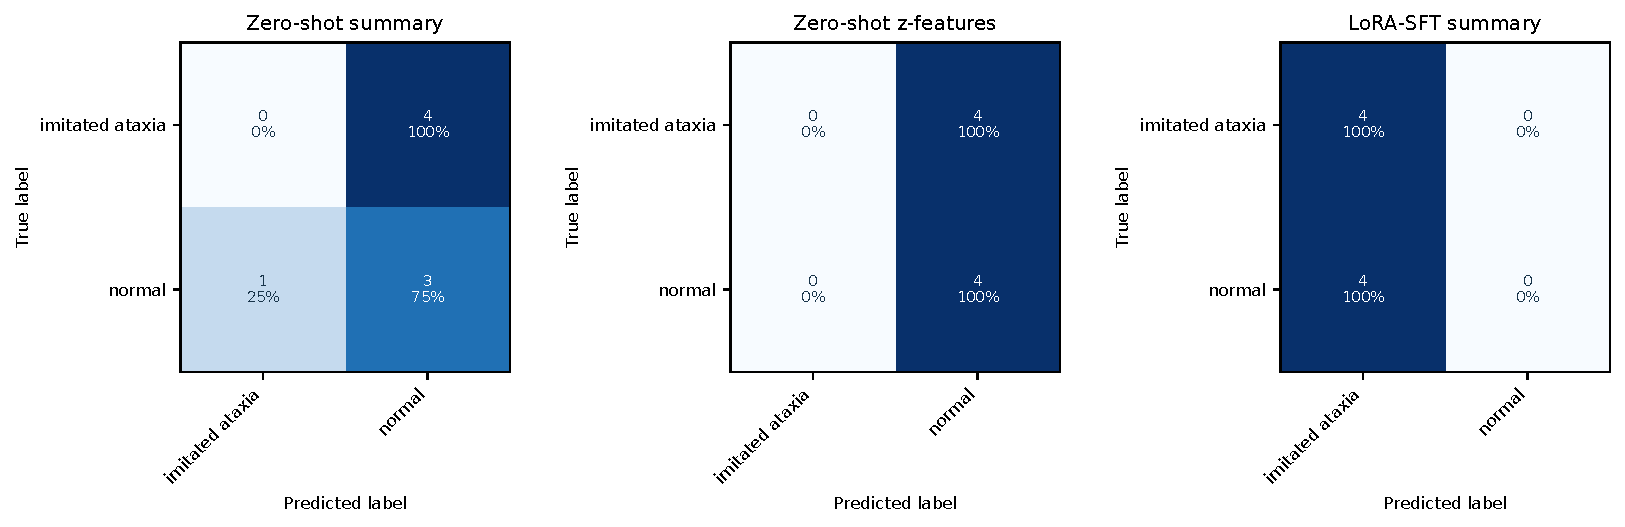
\includegraphics[width=\textwidth]{figures/confusion_ataxia.pdf}
\caption{\textbf{ATAXIA confusion matrices.} Eight clips from four participants make these descriptive rather than rank-defining.}
\label{fig:cm_ataxia}
\end{figure}

\begin{table}[H]
\centering
\caption{\textbf{GMFCS per-class results.} Precision, recall, and F1 are recomputed from committed predictions; all task classes are retained.}
\label{tab:per_class_gmfcs}
\small
\begin{adjustbox}{max width=\textwidth}
\begin{tabular}{llrrrr}
\toprule
Condition & Class & Support & Precision & Recall & F1 \\
\midrule
Zero-shot summary & 1 & 98 & 0.420 & 0.347 & 0.380 \\
Zero-shot summary & 2 & 97 & 0.361 & 0.134 & 0.195 \\
Zero-shot summary & 3 & 57 & 0.352 & 0.772 & 0.484 \\
Zero-shot summary & 4 & 3 & 0.000 & 0.000 & 0.000 \\
Zero-shot z-features & 1 & 98 & 0.000 & 0.000 & 0.000 \\
Zero-shot z-features & 2 & 97 & 0.293 & 0.124 & 0.174 \\
Zero-shot z-features & 3 & 57 & 0.237 & 0.772 & 0.362 \\
Zero-shot z-features & 4 & 3 & 0.036 & 0.333 & 0.065 \\
LoRA-SFT summary & 1 & 98 & 0.611 & 0.592 & 0.601 \\
LoRA-SFT summary & 2 & 97 & 0.514 & 0.557 & 0.535 \\
LoRA-SFT summary & 3 & 57 & 0.745 & 0.719 & 0.732 \\
LoRA-SFT summary & 4 & 3 & 0.000 & 0.000 & 0.000 \\
\bottomrule
\end{tabular}
\end{adjustbox}
\end{table}

\begin{figure}[H]
\centering
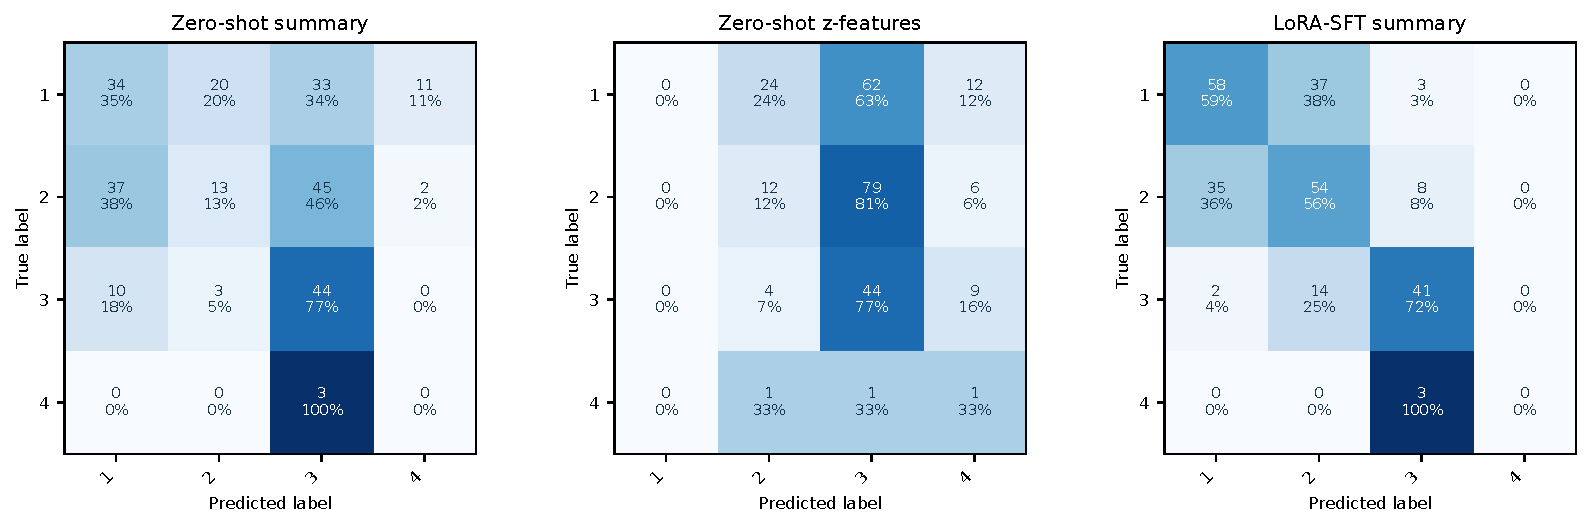
\includegraphics[width=\textwidth]{figures/confusion_gmfcs.pdf}
\caption{\textbf{GMFCS confusion matrices.} SFT improves levels 1--3 but the three level-4 clips are all predicted as level 3.}
\label{fig:cm_gmfcs}
\end{figure}

\begin{table}[H]
\centering
\caption{\textbf{PARKINSONISM per-class S results.} Precision, recall, and F1 are recomputed from committed predictions; all task classes are retained.}
\label{tab:per_class_parkinsonism}
\small
\begin{adjustbox}{max width=\textwidth}
\begin{tabular}{llrrrr}
\toprule
Condition & Class & Support & Precision & Recall & F1 \\
\midrule
Zero-shot summary & mild & 14 & 0.500 & 1.000 & 0.667 \\
Zero-shot summary & severe & 15 & 1.000 & 0.067 & 0.125 \\
Zero-shot z-features & mild & 14 & 0.706 & 0.857 & 0.774 \\
Zero-shot z-features & severe & 15 & 0.833 & 0.667 & 0.741 \\
LoRA-SFT summary & mild & 14 & 0.667 & 0.286 & 0.400 \\
LoRA-SFT summary & severe & 15 & 0.565 & 0.867 & 0.684 \\
\bottomrule
\end{tabular}
\end{adjustbox}
\end{table}

\begin{figure}[H]
\centering
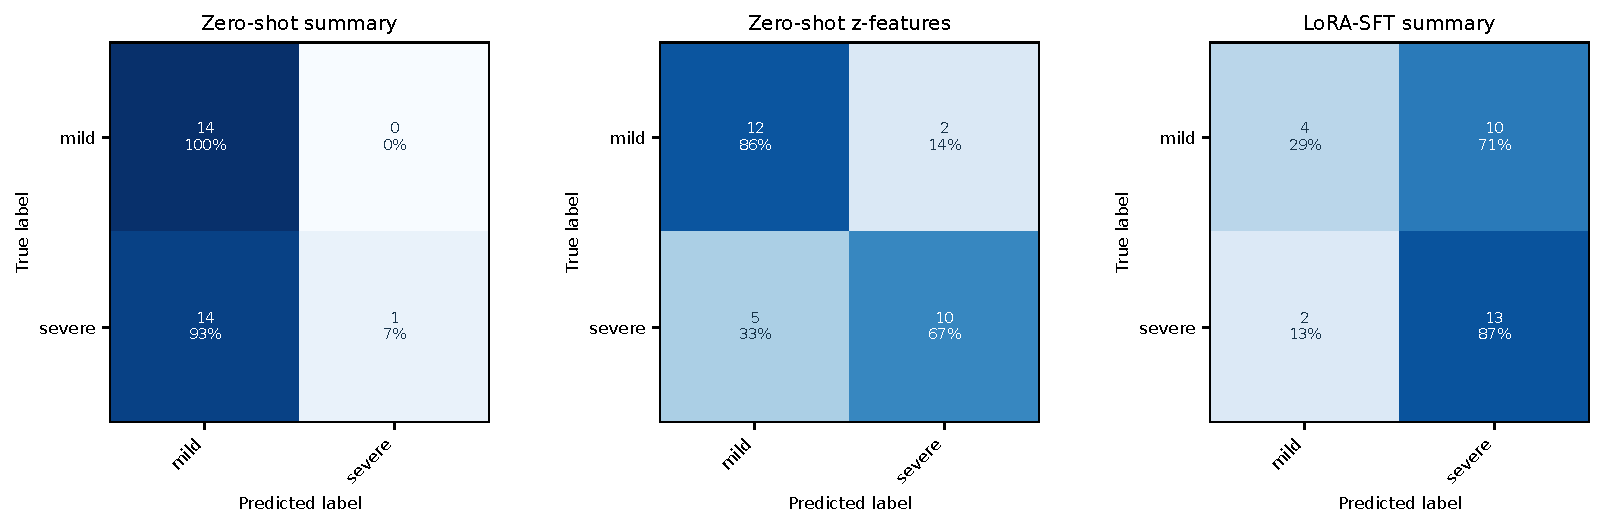
\includegraphics[width=\textwidth]{figures/confusion_parkinsonism.pdf}
\caption{\textbf{PARKINSONISM confusion matrices.} The z-feature view provides the most balanced class recovery in this five-subject test.}
\label{fig:cm_parkinsonism}
\end{figure}

\begin{table}[H]
\centering
\caption{\textbf{PATHOGAIT per-class S results.} Precision, recall, and F1 are recomputed from committed predictions; all task classes are retained.}
\label{tab:per_class_pathogait}
\small
\begin{adjustbox}{max width=\textwidth}
\begin{tabular}{llrrrr}
\toprule
Condition & Class & Support & Precision & Recall & F1 \\
\midrule
Zero-shot summary & antalgic & 240 & 0.000 & 0.000 & 0.000 \\
Zero-shot summary & lurch & 240 & 0.027 & 0.004 & 0.007 \\
Zero-shot summary & normal & 240 & 0.184 & 1.000 & 0.310 \\
Zero-shot summary & steppage & 240 & 0.000 & 0.000 & 0.000 \\
Zero-shot summary & stiff\_legged & 240 & 0.000 & 0.000 & 0.000 \\
Zero-shot summary & trendelenburg & 240 & 0.174 & 0.067 & 0.096 \\
Zero-shot z-features & antalgic & 240 & 0.038 & 0.004 & 0.008 \\
Zero-shot z-features & lurch & 240 & 0.114 & 0.017 & 0.029 \\
Zero-shot z-features & normal & 240 & 0.173 & 0.700 & 0.278 \\
Zero-shot z-features & steppage & 240 & 0.117 & 0.087 & 0.100 \\
Zero-shot z-features & stiff\_legged & 240 & 0.000 & 0.000 & 0.000 \\
Zero-shot z-features & trendelenburg & 240 & 0.428 & 0.408 & 0.418 \\
LoRA-SFT summary & antalgic & 240 & 0.462 & 0.350 & 0.398 \\
LoRA-SFT summary & lurch & 240 & 0.379 & 0.371 & 0.375 \\
LoRA-SFT summary & normal & 240 & 0.720 & 0.558 & 0.629 \\
LoRA-SFT summary & steppage & 240 & 0.319 & 0.438 & 0.369 \\
LoRA-SFT summary & stiff\_legged & 240 & 0.640 & 0.808 & 0.715 \\
LoRA-SFT summary & trendelenburg & 240 & 0.239 & 0.204 & 0.220 \\
\bottomrule
\end{tabular}
\end{adjustbox}
\end{table}

\begin{figure}[H]
\centering
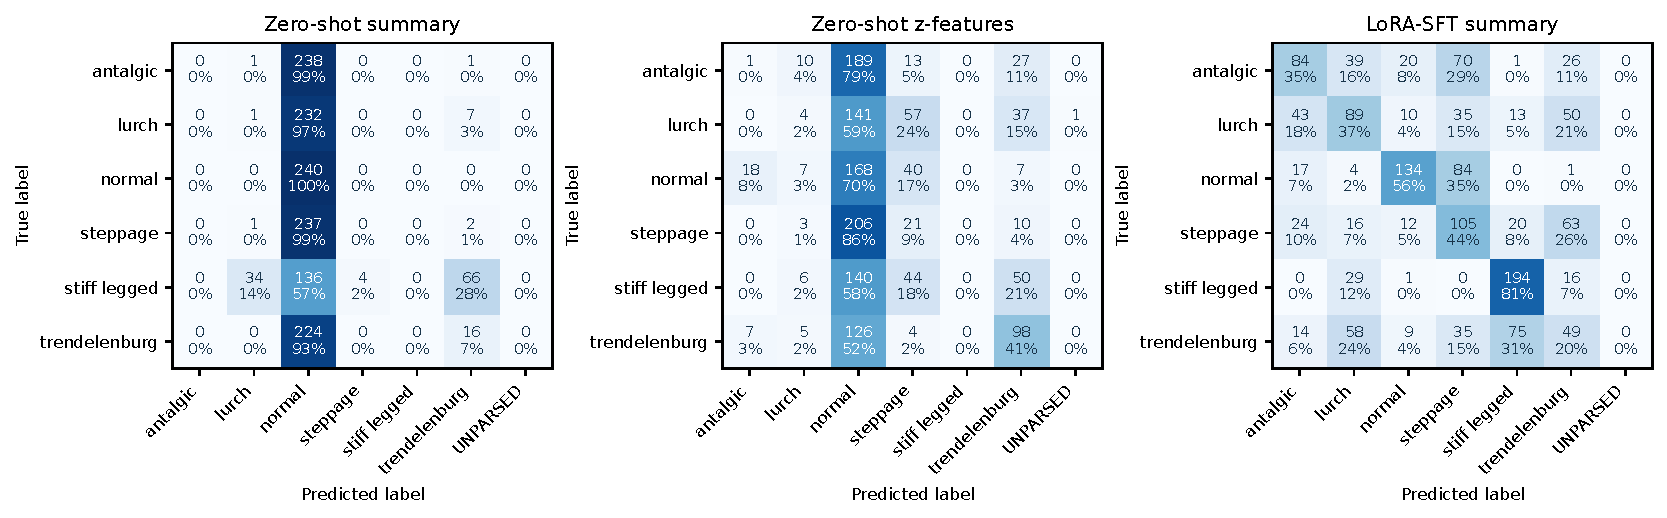
\includegraphics[width=\textwidth]{figures/confusion_pathogait.pdf}
\caption{\textbf{PATHOGAIT confusion matrices.} Zero-shot summary predictions concentrate on normal; SFT distributes predictions across all six patterns but remains uneven, particularly for Trendelenburg gait. The z-feature condition contains one unparsed lurch output, shown as an error.}
\label{fig:cm_pathogait}
\end{figure}

\begin{table}[H]
\centering
\caption{\textbf{ASD-Kinect per-class results.} Precision, recall, and F1 are recomputed from committed predictions; all task classes are retained.}
\label{tab:per_class_asd_kinect}
\small
\begin{adjustbox}{max width=\textwidth}
\begin{tabular}{llrrrr}
\toprule
Condition & Class & Support & Precision & Recall & F1 \\
\midrule
Zero-shot summary & ASD & 10 & 0.000 & 0.000 & 0.000 \\
Zero-shot summary & typically\_developing & 10 & 0.474 & 0.900 & 0.621 \\
Zero-shot z-features & ASD & 10 & 1.000 & 0.100 & 0.182 \\
Zero-shot z-features & typically\_developing & 10 & 0.526 & 1.000 & 0.690 \\
LoRA-SFT summary & ASD & 10 & 0.474 & 0.900 & 0.621 \\
LoRA-SFT summary & typically\_developing & 10 & 0.000 & 0.000 & 0.000 \\
\bottomrule
\end{tabular}
\end{adjustbox}
\end{table}

\begin{figure}[H]
\centering
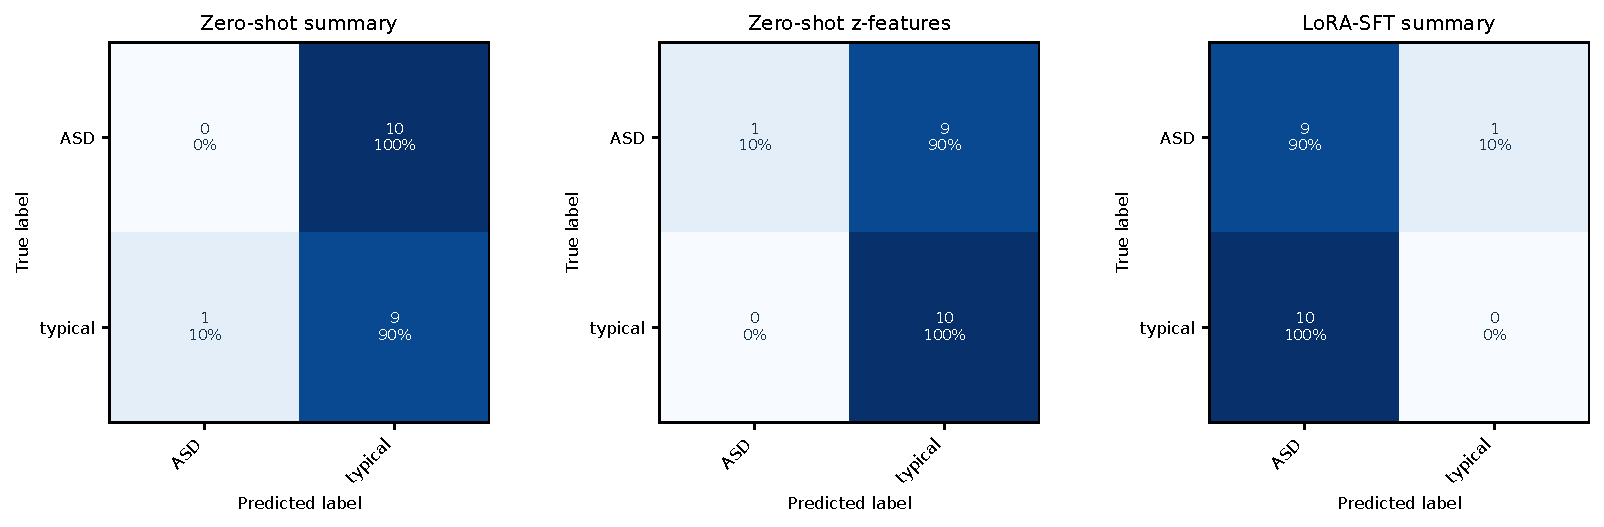
\includegraphics[width=\textwidth]{figures/confusion_asd_kinect.pdf}
\caption{\textbf{ASD-Kinect confusion matrices.} One clip per participant yields 20 independent observations, but the small class supports make all estimates coarse.}
\label{fig:cm_asd}
\end{figure}

\begin{table}[H]
\centering
\caption{\textbf{CARE-PD per-class S results.} Precision, recall, and F1 are recomputed from committed predictions; all task classes are retained.}
\label{tab:per_class_care_pd}
\small
\begin{adjustbox}{max width=\textwidth}
\begin{tabular}{llrrrr}
\toprule
Condition & Class & Support & Precision & Recall & F1 \\
\midrule
Zero-shot summary & 0 & 240 & 0.528 & 0.471 & 0.498 \\
Zero-shot summary & 1 & 247 & 0.455 & 0.490 & 0.472 \\
Zero-shot summary & 2 & 160 & 0.292 & 0.338 & 0.313 \\
Zero-shot summary & 3 & 18 & 0.000 & 0.000 & 0.000 \\
Zero-shot z-features & 0 & 240 & 0.000 & 0.000 & 0.000 \\
Zero-shot z-features & 1 & 247 & 0.310 & 0.073 & 0.118 \\
Zero-shot z-features & 2 & 160 & 0.275 & 0.856 & 0.416 \\
Zero-shot z-features & 3 & 18 & 0.000 & 0.000 & 0.000 \\
LoRA-SFT summary & 0 & 240 & 0.519 & 0.683 & 0.590 \\
LoRA-SFT summary & 1 & 247 & 0.414 & 0.441 & 0.427 \\
LoRA-SFT summary & 2 & 160 & 0.304 & 0.150 & 0.201 \\
LoRA-SFT summary & 3 & 18 & 1.000 & 0.389 & 0.560 \\
\bottomrule
\end{tabular}
\end{adjustbox}
\end{table}

\begin{figure}[H]
\centering
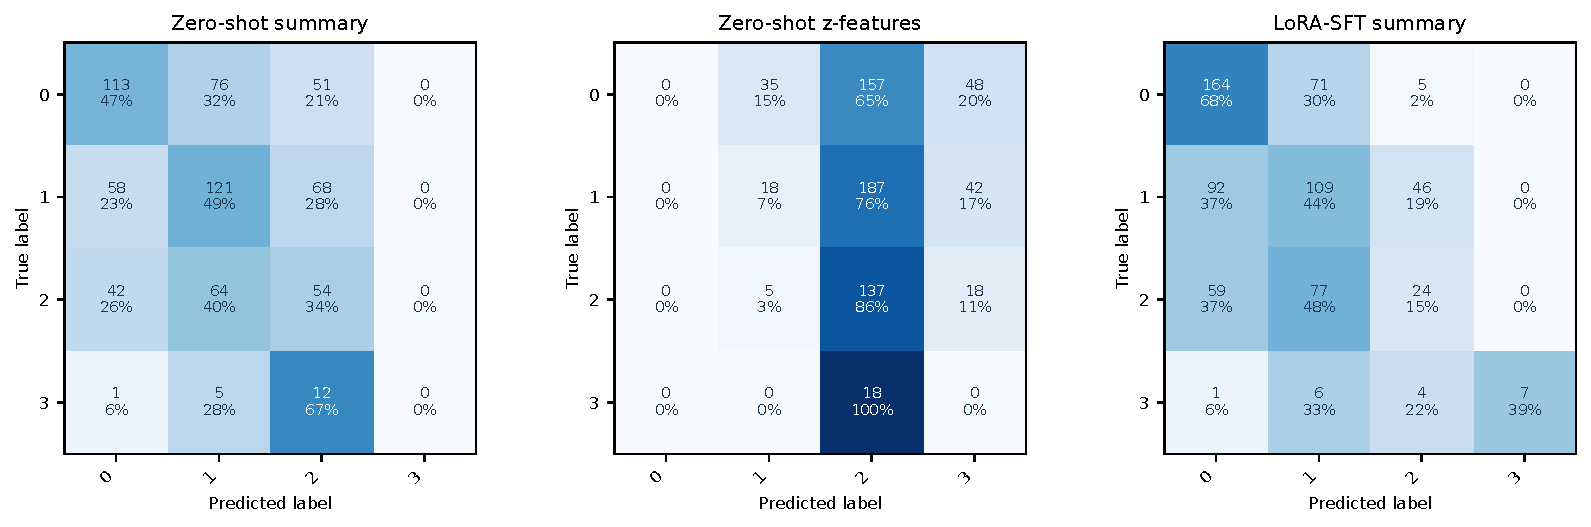
\includegraphics[width=0.86\textwidth]{figures/confusion_care_pd.pdf}
\caption{\textbf{CARE-PD UPDRS-gait confusion matrices.} The evaluation is restricted to scores 0--3 from one task. Score 3 has 18 clips and should not be interpreted as a precise severity-specific estimate.}
\label{fig:cm_care}
\end{figure}

The six confusion analyses refine the aggregate conclusion. Zero-shot failure is frequently a class-allocation failure rather than uniformly low recall: ATAXIA, ASD-Kinect, and PARKINSONISM each approach a single-class decision under at least one view. GMFCS and CARE-PD errors are predominantly adjacent or near-adjacent under SFT, which is reflected by improved ordinal metrics even when macro-F1 remains below the feature references. PATHOGAIT SFT recovers substantial normal and stiff-legged performance but not a balanced six-class mapping.

\subsection{Reproducibility Contract and Evidence Limits}
\label{sec:supp_repro}

The release data model records participant manifests, native/canonical poses, raw/train-scaled features, label-free summaries, prompts, and per-clip predictions. The 55-file shared-condition collection contains raw outputs, summaries, scoring, control, and training code and reference/statistical records. The separate split-repair evidence contains GMFCS participant maps and retrained-model predictions and is not part of that count. Complete source poses, feature/summary input layers, split-generation inputs, adapters, and training logs remain external. The supplied audit checks available predictions and test-record alignment without claiming that full retraining has been reproduced.

The following boundaries apply to all reported conclusions:
\begin{enumerate}
\item GaitEval measures dataset-specified classification grounded in pose-derived evidence; it does not validate autonomous diagnosis, treatment choice, or clinical deployment.
\item ATAXIA and PATHOGAIT contain performed rather than patient gait; CARE-PD uses a task-specific clinical subset, and ASD-Kinect has the source-provenance caveat stated above. These are population limitations within one six-dataset benchmark.
\item Skeleton estimation removes appearance cues but introduces sensor-, estimator-, and layout-specific noise. The deterministic feature set is interpretable but incomplete, and unsigned asymmetry loses laterality.
\item Test cohorts are small for ATAXIA, PARKINSONISM, PATHOGAIT, ASD-Kinect, and the highest ordinal severity classes. Subject-level intervals, per-class support, and confusion matrices must accompany point estimates.
\item In-distribution SFT demonstrates learning of supplied task mappings. It does not by itself show acquisition of transferable clinical knowledge.
\item Cross-condition evidence is restricted to the harmonized ATAXIA--PATHOGAIT pair and combines condition, cohort, sensor, and representation shift. No broader cross-disease transfer conclusion follows.
\end{enumerate}


\subsection{Six-Dataset Experimental Coverage}
\label{sec:supp_six_coverage}

All six datasets are benchmark members under one evaluation protocol. Seven shared Qwen-7B conditions give 42 prediction-backed cells. Two additional raw-feature cells and ten ASD-Kinect/CARE-PD model-comparison cells, plus a separate 12-class CARE-PD diagnostic, give 55 files in this collection. Other model/view/adaptation results are recorded on the test populations stated in their captions. Coordinate prompting, few-shot, feature-SFT, and transfer have the coverage in Table~\ref{supp:tab:coverage_matrix}; benchmark membership does not imply a complete Cartesian product of configurations.

\begin{importtable}
\centering
\caption{\textbf{Experimental coverage across six datasets.} ``Yes'' means a result exists on the stated test set; ``--'' means no result; ``Unverified'' means the corrected records needed to validate a historical result are missing. All six datasets have the seven Qwen-7B conditions and matched LR/SVM. Test counts for each experiment are stated in the result captions and supplemental evaluation-record inventory. The five-model column excludes the Qwen-7B anchor.}
\label{supp:tab:coverage_matrix}
\small
\setlength{\tabcolsep}{4pt}
\resizebox{\textwidth}{!}{%
\begin{tabular}{llllllllll}
\toprule
Dataset & Five families & ZS summary/z & ZS raw feat. & Summary SFT & LR/SVM+controls & Few-shot & Feature SFT & Coordinates & Transfer \\
\midrule
ASD-Kinect & Yes & Yes & Yes & Yes & Yes & -- & -- & -- & -- \\
ATAXIA & Yes & Yes & -- & Yes & Yes & Yes & Yes & Yes & Tested pair \\
CARE-PD & Yes & Yes & Yes & Yes & Yes & -- & -- & -- & -- \\
GMFCS & Yes & Yes & -- & Yes & Yes & -- & -- & Unverified & -- \\
PARKINSONISM & Yes & Yes & -- & Yes & Yes & Yes & -- & Normalized & -- \\
PATHOGAIT & Yes & Yes & -- & Yes & Yes & Yes & Yes & Yes & Tested pair \\
\bottomrule
\end{tabular}}
\end{importtable}

\begin{table}[H]
\centering
\caption{\textbf{Same-feature references for the seven shared conditions.} All six datasets use the features and evaluation records specified for the shared-condition comparisons. CARE-PD is the four-class UPDRS gait task with 665 test clips. The LR/SVM inputs match the corresponding named-feature LLM inputs; $n$ and Subjects identify the evaluated records.}
\label{supp:tab:shared_references}
\small
\setlength{\tabcolsep}{4pt}
\resizebox{\textwidth}{!}{%
\begin{tabular}{lrrrrrrrrr}
\toprule
Dataset & $n$ & Subjects & Chance mF1 & LR Acc. & LR mF1 & LR $\kappa$ & SVM Acc. & SVM mF1 & SVM $\kappa$ \\
\midrule
ASD-Kinect & 20 & 20 & 0.490 & 0.700 & 0.697 & 0.400 & 0.750 & 0.744 & 0.500 \\
ATAXIA & 8 & 4 & 0.488 & 0.875 & 0.873 & 0.750 & 0.875 & 0.873 & 0.750 \\
CARE-PD & 665 & 24 & 0.250 & 0.621 & 0.659 & 0.437 & 0.621 & 0.650 & 0.435 \\
GMFCS & 255 & 149 & 0.250 & 0.639 & 0.579 & 0.458 & 0.647 & 0.571 & 0.469 \\
PARKINSONISM & 29 & 5 & 0.494 & 0.586 & 0.561 & 0.187 & 0.586 & 0.574 & 0.183 \\
PATHOGAIT & 1440 & 2 & 0.166 & 0.881 & 0.881 & 0.858 & 0.897 & 0.897 & 0.877 \\
\bottomrule
\end{tabular}}
\end{table}
\begin{table}[H]
\centering
\caption{\textbf{Six-dataset input-view comparison with Qwen2.5-7B.} Accuracy / macro-F1 / $\kappa$ on identical within-dataset test records: 20/8/665/255/29/1,440 clips in dataset order. Raw-feature runs exist only where shown; ``--'' is an unexecuted configuration. Coordinate prompting was not run on these test sets.}
\label{supp:tab:standardized_views_six}
\small
\setlength{\tabcolsep}{4pt}
\resizebox{\textwidth}{!}{%
\begin{tabular}{lccc}
\toprule
Dataset & Motion summary & Raw named features & Z-scored named features \\
\midrule
ASD-Kinect & 0.450 / 0.310 / $-0.100$ & 0.500 / 0.333 / 0.000 & 0.550 / 0.436 / 0.100 \\
ATAXIA & 0.375 / 0.273 / $-0.250$ & -- & 0.500 / 0.333 / 0.000 \\
CARE-PD & 0.433 / 0.321 / 0.152 & 0.332 / 0.221 / 0.039 & 0.233 / 0.133 / 0.020 \\
GMFCS & 0.357 / 0.265 / 0.099 & -- & 0.224 / 0.150 / $-0.003$ \\
PARKINSONISM & 0.517 / 0.396 / 0.065 & -- & 0.759 / 0.757 / 0.520 \\
PATHOGAIT & 0.178 / 0.069 / 0.014 & -- & 0.203 / 0.139 / 0.043 \\
\bottomrule
\end{tabular}}
\end{table}

\paragraph{Known accepted-version discrepancies.}
The GMFCS source described 899 original test clips, 885 in a resource summary, and 866 after correction. Released maps resolve the original counts as 1,574/473/899 and the repaired counts as 1,602/478/866. Verified corrected values are used for model comparison, SFT, and references. Newly recovered 7B view numbers are shown in red for author review, with their distinct provenance disclosed; matching per-record outputs remain unavailable and no provisional cell is used in scientific comparisons. The seven-condition experiment has 255 test clips from 149 participants and an incomplete released training manifest. CARE-PD primary references use 665 clips/four labels; the 970-clip/12-label reference is a different task and excluded. Normalized result records and generated checks take precedence over stale source Markdown.

\paragraph{Prompt and parser settings.}
The recorded \texttt{view\_run.py} template contains a 3D-skeleton/biomechanical-dimension preamble; \texttt{v21\_llm\_runner.py} renders the seven-condition evidence with a shorter skeleton-sequence preamble. The former parser has a unique truncated-label-prefix fallback; the latter requires complete boundary-anchored candidates. These implementation settings remain attached to their actual outputs. Scores are not substituted across different prompts, test records, or parsers, and missing experiments remain unreported.

\paragraph{Evidence assets still unavailable.}
The collection includes committed results and corrective reruns. This revision executes no new training or inference. Complete records, pose/feature/summary layers, and training artifacts are required for end-to-end reproduction. A canonical 19-joint data layer does not establish that the 12-joint coordinate-input configuration was run on every evaluated record set.

\paragraph{Recomputed binary-label identity.}
ASD-Kinect uses the positive label \texttt{ASD}. Recomputing from the committed shared-condition predictions gives summary sensitivity/specificity 0.000/0.900, z-feature 0.100/1.000, and summary-SFT 0.900/0.000. These numerical values agree with the accepted binary-metric table; the regenerated table preserves them and standardizes the displayed label identity. This is a consistency check, not a correction to the accepted binary scores or an extra experiment.

\clearpage
\section{Complete Results by Experimental Setting}
\begin{importtable}
\centering
\caption{\textbf{Five-model zero-shot motion-summary benchmark.} Accuracy / macro-F1 / Cohen's $\kappa$ for ASD-Kinect/ATAXIA/CARE-PD/GMFCS/PARKINSONISM/PATHOGAIT, respectively. These test sets also define the supervision ladder; their sizes differ from the seven-condition comparison where indicated. Bold marks the highest macro-F1 per dataset; invalid outputs count as errors.}
\label{v2detail:tab:zero_shot_full}
\small
\setlength{\tabcolsep}{4pt}
\resizebox{\textwidth}{!}{
\begin{tabular}{lccccc}
\toprule
\textbf{Dataset (Maj. Acc.)}
& \textbf{Llama-3.3-70B}
& \textbf{Qwen2.5-72B}
& \textbf{Gemma-3-27B}
& \textbf{GLM-4-32B}
& \textbf{DeepSeek-R1-32B} \\
\midrule
ASD-Kinect (0.500)
& 0.500 / 0.451 / 0.000
& 0.450 / 0.373 / $-0.100$
& 0.450 / 0.310 / $-0.100$
& 0.450 / 0.373 / $-0.100$
& 0.600 / \textbf{0.583} / 0.200 \\
ATAXIA (0.686)
& 0.686 / 0.407 / 0.000
& 0.685 / 0.406 / $-0.002$
& 0.686 / 0.407 / 0.000
& 0.686 / 0.407 / 0.000
& 0.684 / \textbf{0.408} / $-0.002$ \\
CARE-PD (0.361)
& 0.441 / 0.262 / 0.119
& 0.445 / 0.268 / 0.129
& 0.439 / 0.249 / 0.113
& 0.441 / \textbf{0.350} / 0.124
& 0.398 / 0.295 / 0.099 \\
GMFCS (0.356)
& 0.353 / 0.212 / 0.025
& 0.372 / \textbf{0.222} / 0.043
& 0.313 / 0.163 / 0.030
& 0.269 / 0.127 / $-0.000$
& 0.311 / 0.191 / 0.014 \\
PARKINSONISM (0.583)
& 0.583 / 0.368 / 0.000
& 0.575 / \textbf{0.472} / 0.035
& 0.583 / 0.368 / 0.000
& 0.583 / 0.368 / 0.000
& 0.583 / 0.368 / 0.000 \\
PATHOGAIT (0.226)
& 0.159 / 0.062 / $-0.010$
& 0.155 / 0.055 / $-0.009$
& 0.165 / 0.047 / $-0.001$
& 0.141 / 0.069 / $-0.069$
& 0.166 / \textbf{0.094} / $-0.007$ \\
\bottomrule
\end{tabular}}
\end{importtable}

\begin{importtable}
\centering\small
\caption{\textbf{Shared six-dataset evidence-use and adaptation evaluation.} Macro-F1 point estimates use the fixed task label set. Bracketed participant-cluster intervals and paired bootstrap tail areas $p$ are archived statistics with the historical resampling convention described in Methods; they are not newly recomputed fixed-label intervals. $\Delta_{\rm ShufEv}$ is summary zero-shot minus shuffled evidence; $\Delta_{\rm SFT}$ is summary-SFT minus summary zero-shot within Qwen2.5-7B. PATHOGAIT has only two test participants, so its values are descriptive and intervals/$p$ are withheld.}
\label{v22:tab:evidence_use}
\setlength{\tabcolsep}{3pt}
\begin{adjustbox}{max width=\linewidth}
\begin{tabular}{llrlllll}\toprule
Dataset & Task & Clips (subjects) & Chance & LR [95\% CI] & 7B ZS [95\% CI] & $\Delta_{\rm ShufEv}$ ($p$) & 7B SFT ($\Delta_{\rm SFT}$, $p$)\\\midrule
ASD-Kinect & binary & 20 (20) & .490 & .697 [.479, .890] & .310 [.200, .394] & $-.125$ (.25) & .310 (.000, 1.0)\\
ATAXIA & binary, imitated & 8 (4) & .488 & .873 [.564, 1.000] & .273 [.111, .333] & .000 (1.0) & .333 (+.061, .60)\\
CARE-PD & UPDRS gait 0--3 & 665 (24) & .250 & .659 [.407, .742] & .321 [.262, .404] & +.065 (.029) & .445 (+.124, .43)\\
GMFCS & four-level ordinal & 255 (149) & .250 & .579 [.474, .662] & .265 [.217, .308] & +.052 (.089) & .467 (+.202, .001)\\
PARKINSONISM & binary severity & 29 (5) & .494 & .561 [.416, .654] & .396 [.222, .530] & +.086 (.14) & .542 (+.146, .47)\\
PATHOGAIT & six-class, simulated & 1440 (2) & .166 & .881 & .069 & $-.002$ & .451 (+.382)\\\bottomrule
\end{tabular}
\end{adjustbox}
\end{importtable}

\begin{importtable}
\centering
\caption{\textbf{Four input-view families and a feature-scaling control.} Accuracy / macro-F1 / $\kappa$. Z-scoring is an encoding of the named features. ``--'' means no recoverable numeric result.}
\label{v2detail:tab:modality_ablation}
\small
\setlength{\tabcolsep}{2pt}
\renewcommand{\arraystretch}{0.9}
\resizebox{\textwidth}{!}{
\begin{tabular}{lcccccc}\toprule
\textbf{Input view} & \textbf{ASD-Kinect} & \textbf{ATAXIA} & \textbf{CARE-PD} & \textbf{GMFCS} & \textbf{PARKINSONISM} & \textbf{PATHOGAIT}\\\midrule
Raw coordinates$^{\dagger}$ & -- & 0.573 / 0.323 / 0.009 & -- & -- & -- & 0.093 / 0.083 / 0.038\\
Normalized coordinates & -- & 0.316 / 0.244 / 0.002 & -- & 0.282 / 0.110 / 0.000 & 0.442 / 0.441 / $-0.095$ & 0.110 / 0.034 / 0.000\\
Motion summary & 0.450 / 0.310 / $-0.100$ & 0.692 / 0.452 / 0.046 & 0.433 / 0.321 / 0.152 & 0.259 / 0.113 / $-0.009$ & 0.550 / 0.400 / $-0.045$ & 0.142 / 0.087 / $-0.024$\\
Named feature vector & 0.500 / 0.333 / 0.000 & 0.382 / 0.347 / 0.057 & 0.332 / 0.221 / 0.039 & 0.343 / 0.245 / 0.007 & 0.417 / 0.294 / 0.000 & 0.110 / 0.033 / 0.000\\
Z-scored named feature vector & 0.550 / 0.436 / 0.100 & 0.583 / \textbf{0.495} / $-0.008$ & 0.233 / 0.133 / 0.020 & 0.185 / 0.100 / $-0.049$ & 0.508 / \textbf{0.493} / $-0.014$ & 0.150 / \textbf{0.130} / $-0.011$\\
\bottomrule
\end{tabular}}
\end{importtable}

\begin{importtable}
\centering
\caption{\textbf{Six-dataset input-view comparison with Qwen2.5-7B.} Accuracy / macro-F1 / $\kappa$ on identical within-dataset test records: 20/8/665/255/29/1,440 clips in dataset order. Raw-feature runs exist only where shown; ``--'' is an unexecuted configuration. Coordinate prompting was not run on these test sets.}
\label{v2detail:tab:standardized_views_six}
\small
\setlength{\tabcolsep}{4pt}
\resizebox{\textwidth}{!}{%
\begin{tabular}{lccc}
\toprule
Dataset & Motion summary & Raw named features & Z-scored named features \\
\midrule
ASD-Kinect & 0.450 / 0.310 / $-0.100$ & 0.500 / 0.333 / 0.000 & 0.550 / 0.436 / 0.100 \\
ATAXIA & 0.375 / 0.273 / $-0.250$ & -- & 0.500 / 0.333 / 0.000 \\
CARE-PD & 0.433 / 0.321 / 0.152 & 0.332 / 0.221 / 0.039 & 0.233 / 0.133 / 0.020 \\
GMFCS & 0.357 / 0.265 / 0.099 & -- & 0.224 / 0.150 / $-0.003$ \\
PARKINSONISM & 0.517 / 0.396 / 0.065 & -- & 0.759 / 0.757 / 0.520 \\
PATHOGAIT & 0.178 / 0.069 / 0.014 & -- & 0.203 / 0.139 / 0.043 \\
\bottomrule
\end{tabular}}
\end{importtable}

\begin{importtable}
\centering
\caption{\textbf{Same-feature linear references for the model/view experiments.} Accuracy, macro-F1, and Cohen's $\kappa$; test sizes are given in the final column. Chance mF1 is the recorded stratified-chance reference. Bold marks the stronger linear reference per metric. These references match the feature inputs and test populations of the supervision ladder; the next table gives references for the seven shared conditions.}
\label{v2detail:tab:linear_references}
\small
\setlength{\tabcolsep}{3.2pt}
\resizebox{\textwidth}{!}{
\begin{tabular}{lcccccccccc}
\toprule
\textbf{Dataset}
& \textbf{Classes}
& \textbf{Maj. Acc.}
& \textbf{Chance mF1}
& \textbf{LR Acc.}
& \textbf{LR mF1}
& \textbf{LR $\kappa$}
& \textbf{SVM Acc.}
& \textbf{SVM mF1}
& \textbf{SVM $\kappa$}
& $\boldsymbol{n_{\mathrm{te}}}$ \\
\midrule
ASD-Kinect
& 2
& 0.500
& 0.490
& 0.700
& 0.697
& 0.400
& 0.750
& 0.744
& 0.500
& 20 \\

ATAXIA
& 2
& 0.686
& 0.498
& \textbf{0.778}
& \textbf{0.763}
& \textbf{0.533}
& 0.774
& 0.759
& 0.524
& 1647 \\

CARE-PD
& 4
& 0.361
& 0.250
& 0.621
& 0.659
& 0.437
& 0.621
& 0.650
& 0.435
& 665 \\

GMFCS
& 4
& 0.356
& 0.250
& 0.461
& 0.395
& 0.241
& \textbf{0.492}
& \textbf{0.412}
& \textbf{0.271}
& 866 \\

PARKINSONISM
& 2
& 0.583
& 0.499
& \textbf{0.625}
& \textbf{0.613}
& \textbf{0.226}
& 0.600
& 0.583
& 0.168
& 120 \\

PATHOGAIT
& 6
& 0.226
& 0.166
& \textbf{0.659}
& \textbf{0.662}
& \textbf{0.589}
& 0.656
& 0.644
& 0.585
& 2181 \\
\bottomrule
\end{tabular}}
\end{importtable}

\begin{importtable}
\centering
\caption{\textbf{Same-feature references for the seven shared conditions.} All six datasets use the features and evaluation records specified for the shared-condition comparisons. CARE-PD is the four-class UPDRS gait task with 665 test clips. The LR/SVM inputs match the corresponding named-feature LLM inputs; $n$ and Subjects identify the evaluated records.}
\label{v2detail:tab:shared_references}
\small
\setlength{\tabcolsep}{4pt}
\resizebox{\textwidth}{!}{%
\begin{tabular}{lrrrrrrrrr}
\toprule
Dataset & $n$ & Subjects & Chance mF1 & LR Acc. & LR mF1 & LR $\kappa$ & SVM Acc. & SVM mF1 & SVM $\kappa$ \\
\midrule
ASD-Kinect & 20 & 20 & 0.490 & 0.700 & 0.697 & 0.400 & 0.750 & 0.744 & 0.500 \\
ATAXIA & 8 & 4 & 0.488 & 0.875 & 0.873 & 0.750 & 0.875 & 0.873 & 0.750 \\
CARE-PD & 665 & 24 & 0.250 & 0.621 & 0.659 & 0.437 & 0.621 & 0.650 & 0.435 \\
GMFCS & 255 & 149 & 0.250 & 0.639 & 0.579 & 0.458 & 0.647 & 0.571 & 0.469 \\
PARKINSONISM & 29 & 5 & 0.494 & 0.586 & 0.561 & 0.187 & 0.586 & 0.574 & 0.183 \\
PATHOGAIT & 1440 & 2 & 0.166 & 0.881 & 0.881 & 0.858 & 0.897 & 0.897 & 0.877 \\
\bottomrule
\end{tabular}}
\end{importtable}

\begin{importtable}
\centering
\caption{\textbf{Task-specific adaptation ladder.} LLM cells are macro-F1 / Cohen's $\kappa$; references are macro-F1. Zero-shot/few-shot use Qwen2.5-72B, while the 7B anchor and SFT use Qwen2.5-7B. Test clips in dataset order are 20/1,647/665/866/120/2,181. PATHOGAIT few-shot instead uses 600 clips, so that change is not a paired full-test gain. GMFCS uses corrected training/test partitions; its matching 7B zero-shot anchor is unverified and withheld. ``--'' denotes unavailable configurations. Bold feature-SFT matches or exceeds the stronger reference point estimate.}
\label{v2detail:tab:adaptation_ladder}
\small
\setlength{\tabcolsep}{4.2pt}
\begin{adjustbox}{max width=\linewidth}
\begin{tabular*}{\textwidth}{@{\extracolsep{\fill}}lccccccc@{}}
\toprule
\textbf{Dataset}
& \textbf{Zero-shot}
& \textbf{Zero-shot (7B)}
& \textbf{Few-shot}
& \textbf{SFT: summary}
& \textbf{SFT: features}
& \textbf{SVM}
& \textbf{LogReg} \\
\midrule
ASD-Kinect
& 0.373 / $-0.100$
& 0.310 / $-0.100$
& --
& 0.310 / $-0.100$
& --
& 0.744
& 0.697 \\

ATAXIA
& 0.406 / $-0.002$
& 0.452 / 0.046
& 0.697 / 0.395
& 0.751 / 0.507
& 0.762 / 0.528
& 0.759
& 0.763 \\

CARE-PD
& 0.268 / 0.129
& 0.321 / 0.152
& --
& 0.445 / 0.168
& --
& 0.650
& 0.659 \\

GMFCS
& 0.222 / 0.043
& --
& --
& 0.259 / 0.043
& --
& 0.412
& 0.395 \\
PARKINSONISM
& 0.472 / 0.035
& 0.400 / $-0.045$
& 0.561 / 0.188
& 0.454 / 0.065
& --
& 0.583
& 0.613 \\

PATHOGAIT
& 0.055 / $-0.009$
& 0.087 / $-0.024$
& 0.185 / 0.081
& 0.609 / 0.511
& \textbf{0.687 / 0.611}
& 0.644
& 0.662 \\

\bottomrule
\end{tabular*}
\end{adjustbox}
\end{importtable}

\begin{importsmalltable}
\centering
\caption{\textbf{Bidirectional ATAXIA--PATHOGAIT transfer.} Models use z-scored feature descriptions; target-majority values are accuracy / macro-F1. Target tests have 2,181 PATHOGAIT clips or 1,647 ATAXIA clips. PATHOGAIT is binarized, so its in-distribution $\kappa$ is not comparable with the six-class adaptation result. OOD denotes target-dataset evaluation. Only this task-compatible pair was tested.}
\label{v2detail:tab:cross_condition_transfer}
\small
\setlength{\tabcolsep}{3.6pt}
\resizebox{\linewidth}{!}{
\begin{tabular}{lccc}
\toprule
\textbf{Train $\rightarrow$ Test}
& \textbf{In-dist. $\kappa$}
& \textbf{OOD Acc. / mF1 / $\kappa$}
& \textbf{Target majority} \\
\midrule
ATAXIA $\rightarrow$ PATHOGAIT
& 0.549
& 0.656 / 0.496 / 0.057
& 0.890 / 0.471 \\

PATHOGAIT $\rightarrow$ ATAXIA
& 0.917
& 0.686 / 0.407 / 0.000
& 0.686 / 0.407 \\
\bottomrule
\end{tabular}}
\end{importsmalltable}


\clearpage
\section{Source examples and release boundary}
Figure 1 illustrates source resources rather than the evaluated test clips. No RGB images are supplied to the text-only models. The source publications and their original references in the main paper remain the attribution basis. Derived plots and vector diagrams are newly drawn; source-example crops retain their separate attribution and license notes in the project repository.

The six-dataset scoring package reproduces point estimates from committed predictions. Reported reference scores and archived cluster-bootstrap outputs are preserved as source measurements, not claimed to be retrained or independently regenerated without their inputs. Full source pose, feature, summary, and split files and adapters are required for end-to-end inference/training reproduction. The code validates participant separation when those split files are supplied and fails on missing, empty, or overlapping inputs.

\paragraph{Resource-example credits.}
ASD-Kinect uses a cropped frame at 0.5\,s from the original \texttt{Svideo.avi}, child-ASD/1/video, in the official \href{https://zenodo.org/records/4025120}{Zenodo archive}. ATAXIA uses captured-video illustrations from Khalil et al., \emph{Diagnosis of Cerebellar Ataxia Based on Gait Analysis Using Human Pose Estimation}, IEEE IECBES2022 (DOI:10.1109/IECBES54088.2022.10079396). CARE-PD uses a crop of the official \href{https://neurips2025.care-pd.ca/static/images/benchmark.png}{benchmark input-mesh example}. GMFCS uses a newly rendered skeleton from \href{https://github.com/stanfordnmbl/mobile-gaitlab}{mobile-gaitlab}'s public demo keypoints (frame60), not confirmed as an evaluated participant. PARKINSONISM uses a cropped recording illustration from Deng et al., \emph{npj Parkinson's Disease}10,122(2024), DOI:10.1038/s41531-024-00742-x (CC BY4.0). PATHOGAIT renders recorded joints from the \href{https://github.com/kooksung/pathological_gait_datasets}{official source repository}. Crops and skeleton renderings were made for this overview. These are resource illustrations, not clip-matched model evidence. Source-paper image reuse terms and any unlicensed derived display must be confirmed before final distribution; dataset availability alone does not establish image permission.

\section{Reviewer-requested qualitative examples}
\begin{table}[H]\centering\small
\caption{Prediction-backed qualitative decisions across all six datasets. Outputs are verbatim from committed logs. No matching pose or prompt is inferred.}
\begin{tabular}{llll}\toprule Dataset / view & True label & Raw output & Correct\\\midrule
asd\_kinect / zs & typically\_developing & typically\_developing & yes\\
asd\_kinect / zs & ASD & typically\_developing & no\\
ataxia / zs & normal & normal & yes\\
ataxia / zs & mimicked\_ataxia & normal & no\\
care\_pd / zs & 0 & UPDRS gait score 0 & yes\\
care\_pd / zs & 1 & UPDRS gait score 0 & no\\
gmfcs / zs & 3 & GMFCS level 3 & yes\\
gmfcs / zs & 2 & GMFCS level 1 & no\\
parkinsonism / zs & severe & severe & yes\\
parkinsonism / zs & severe & mild & no\\
pathogait / zs & normal & normal & yes\\
pathogait / zs & antalgic & normal & no\\
\bottomrule\end{tabular}\end{table}
For each dataset, the examples are deterministic selections from the committed predictions, showing one correct and one incorrect summary or z-feature decision where available. Raw model outputs are shown verbatim; true labels are evaluation annotations, not model-visible metadata. These diagnostics are not representative sampling and do not establish reasoning faithfulness. The original shared-condition input prompts and matching pose records are absent, so no numerical evidence is reconstructed or invented for these cases. Those outputs are therefore not complete matched-input panels.

\clearpage
\section{Recovered Corrective Experiments}
\label{sec:supp_recovered_corrections}

This section incorporates corrective experiments that were already executed and released by the authors. It does not report new training performed for this revision. The correction package records source commits \texttt{2348b11} of the private working archive and \texttt{60f3503} of the public GaitEval repository. The verification script recomputes split intersections, exact test-ID alignment, raw-output parsing, SFT point metrics, and the corrected evaluation-record joins. Archived reference-model and bootstrap values are identified as such rather than represented as independently retrained here.

\subsection{GMFCS: Original and Corrected Participant Partitions}
The original partition contains 1,574/473/899 train/validation/test clips. Its original-to-corrected index maps assign a participant to the first split in training--validation--test order in which that participant appears, and then move all that participant's clips to that split. The rule preserves source clips and yields 1,602/478/866 clips from 94/84/166 participants. Direct intersections of every pair of released participant sets are empty. In particular, the 866 corrected test records correspond to participants absent from both training and validation. The released SFT output IDs are exactly this test set and their true labels match the original indexed records.

The linear references and summary-SFT were rerun on corrected training data. Cached zero-shot summary generations were instead restricted to the corrected test IDs and re-parsed; this is appropriate for those deterministic, non-fitted summary prompts. The archived corrected SFT-minus-LR participant-bootstrap difference is $-0.1367$, interval $[-0.1862,-0.0853]$, paired tail area 0.0010. Source features and per-record reference predictions are needed to independently regenerate that bootstrap. This archived result is distinct from the independently rescored SFT point estimate.

\begin{table}[H]
\centering\small
\caption{\textbf{GMFCS original versus corrected split evidence.} Values are accuracy / macro-F1 / $\kappa$. Reference rows and original rows are archived source measurements; the corrected SFT row is independently recomputed from the supplied generations. The original and corrected SFT rows have different test sets. These use 866 test clips; the seven-condition comparison uses 255.}
\label{tab:supp_repair_details}
\begin{tabular}{lll}\toprule
Experiment & Original: 899 clips & Corrected: 866 clips\\\midrule
72B zero-shot summary & .3693 / .2182 / .0325 & .3718 / .2216 / .0426\\
7B summary-SFT & .3626 / .2553 / .0298 & .3730 / .2585 / .0431\\
Balanced LR & .4516 / .3875 / .2290 & .4607 / .3952 / .2409\\
Balanced SVM & .4917 / .4101 / .2706 & .4919 / .4121 / .2708\\\bottomrule
\end{tabular}
\end{table}

The corrected five-model rows consistently use 866 GMFCS test IDs. Recovered summary/raw-feature/z-feature aggregates refer to 899 clips; normalized-coordinate outputs also lack independently verified corrected IDs. The newly displayed red summary instead uses a logged 866-clip cross-stack run. All four red GMFCS view cells are provisional and excluded from matched-test comparisons. Corrected participant maps apply to the 866-clip experiment. The 255-clip/149-participant, 16-feature shared-condition experiment still requires its full training input manifest for independent separation checks. These two recorded test populations are never treated as interchangeable estimates.

\paragraph{7B view lineage audit.}
\textcolor{red}{For this author-review draft, the source experiment log dated 2026-10-19 reports a separate 866-clip Qwen2.5-7B zero-shot summary run on the bigpurple serving stack: 0.2587 / 0.1129 / $-0.0089$. Its per-record outputs have not been recovered, so it is shown provisionally rather than substituted into the verified supervision ladder. The red raw/z-feature entries below use the historical 899-clip aggregates; the normalized-coordinate entry retains its unverified source-draft status. PATHOGAIT's red named-feature entry is recovered from \texttt{zeroshot-feat-qwen7b\_pathological} in \texttt{r2\_recompute\_part1.json}: all 2,181 outputs are valid, all predict normal gait, and the aggregate is 0.110041 / 0.033044 / 0.000000. Its launcher specifies the base Qwen2.5-7B-Instruct model, test split, unscaled feature-vector input, flat prompt, and 16 output tokens. The previous table generator searched only the alternative \texttt{zs7b\_feature\_vector} name and omitted this run.}
The recovered \texttt{r2\_recompute\_part1.json} associates the following values with the original 899-clip split. Raw per-record generations for these view runs were not recovered, so a corrected 866-clip score cannot be reconstructed from aggregate statistics. In particular, the historical 0.110 summary macro-F1 must not serve as a same-test zero-shot anchor for corrected SFT at 0.2585. The normalized-coordinate cell (0.282 / 0.110 / 0.000) has only a source-draft corrected-split claim and is likewise unverified.
\begin{table}[H]\centering\small
\caption{\textbf{Historical GMFCS 7B views, not corrected-split results.} All three rows have $N=899$ in the source recompute. They are excluded from corrected comparisons.}
\label{tab:gmfcs_view_lineage}
\begin{tabular}{lrrr}\toprule
View & Accuracy & Macro-F1 & $\kappa$\\\midrule
Summary & .2492 & .1097 & $-.0077$\\
Raw named features & .3426 & .2453 & .0066\\
Z-scored features & .1846 & .0999 & $-.0488$\\\bottomrule
\end{tabular}\end{table}

\subsection{PATHOGAIT: Feature-SFT without Valid-Frame Fraction}
The recovered generator removes the line named \texttt{valid\_frame\_fraction} from each feature-view record and asserts removal in every row. Remaining text, IDs, labels, and ordering are preserved. Its SFT data builder accepts \texttt{feature\_vector\_novff}. The source experiment log records the rerun and its training recipe, as well as a change of runtime environment. Full source input layers and training artifacts are external; the public predictions permit an independent check of the paired evaluation records and reported point estimates.

\begin{table}[H]
\centering\small
\caption{\textbf{PATHOGAIT feature-removal evaluation.} Independently rescored generations on identical 2,181 test IDs and true labels; both have zero invalid outputs. The two test participants and single training realization limit inference.}
\label{tab:supp_novff}
\begin{tabular}{lrrr}\toprule
Feature-SFT input & Accuracy & Macro-F1 & $\kappa$\\\midrule
With valid-frame fraction & .6777 & .6870 & .6108\\
Without valid-frame fraction & .6410 & .6316 & .5649\\\bottomrule
\end{tabular}
\end{table}

The macro-F1 change is $-0.0554$ on matching test IDs. The ablated point estimate exceeds quality-free LR/SVM .564/.560, but two participants and one training realization preclude a population-level superiority claim. Runtime changes also prevent causal attribution of the whole difference to the field. The seven shared conditions exclude capture-quality features and use 1,440 PATHOGAIT clips; they contain no feature-SFT result.

\subsection{Release Scope and Source Rights}
The correction bundle supplies split maps, checked generations, code snapshots, and verification code alongside the six-dataset scoring release. Full recordings, adapters, and complete shared-condition inputs remain external. Code/output licensing does not establish dataset or image rights; source credits list outstanding checks.
